%%%%%%%%%%%%%%%%%%%%%%%%%%%%%%%%%%%%%%%%%%%%%%%%%%%%%%%%%%%%%%%%%%%%%%%%%%%%%%%%
%									Chapter 7								   %
%%%%%%%%%%%%%%%%%%%%%%%%%%%%%%%%%%%%%%%%%%%%%%%%%%%%%%%%%%%%%%%%%%%%%%%%%%%%%%%%
\chapter{Gradient Visualization for General Characterization in Profiling Attack}
\label{chap:gradient_viz}
This chapter is inspired from the poster presented at \textsc{Ches} 2018~\cite{masure_understanding_2018} and the paper published at \textsc{Cosade} 2019 in collaboration with Cécile Dumas and Emmanuel Prouff~\cite{masure_gradient_2019}.
This work has benefited from fruitful discussions with Élie Bursztein and Rémi Audebert.
\minitoc
\newpage
%%%%%%%%%%%%%%%%%%%%%%%%%%%%%%%%%%%%%%%%%%%%%%%%%%%%%%%%%%%%%%%%%%%%%%%%%%%%%%%%
\section{Introduction}
    \label{sec:intro_cosade}
    %%%%%%%%%%%%%%%%%%%%%%%%%%%%%%%%%%%%%%%%%%%%%%%%%%%%%%%%%%%%%%%%%%%%%%%%%%%%%%%%
%                   INTRO CHAPTER 6                                            %
%%%%%%%%%%%%%%%%%%%%%%%%%%%%%%%%%%%%%%%%%%%%%%%%%%%%%%%%%%%%%%%%%%%%%%%%%%%%%%%%
In \autoref{sec:counter-measures}, when presenting the different counter-measures that a developer can use to protect an implementation against \gls{sca}, we essentially focused on two criteria:
\begin{enumerate}
    \item the resulting protected implementation must still remain acceptable for the final user, in particular in terms of runtime and memory;
    \item it must guarantee, formally or empirically, the security level requested by the final user or the developer.
\end{enumerate}
Finding the counter-measure meeting those two constraints, often antagonist, is somehow the holy-grail quest of developers willing to prevent \gls{sca} on their devices.

We have seen for example that group-based secret-sharing schemes are able to meet the second condition, to the detriment of the first one.
However, we have not discussed yet in this thesis a third condition, namely how a developer can easily turn an unprotected code into a protected one.
Indeed, although encryption standards such as \gls{aes} are designed to be easily implemented, their specifications do not take into account the development cost of versions protected against \gls{sca}.
In practice, this third constraint turned out to be critical, because it required so far a careful hand-made protection of every possible sensitive intermediate state of the machine running the primitive at a low level -- \ie{} assembly or hardware.

Some recent works propose ways to automatize the secret-sharing of sensitive intermediate computations~\cite{belaid_tornado_2020,belleville_maskara_2020}, with the hope to decrease the developer's hand-made design.
The interest of this approach is thereby to combine this automated generation with a provable security assessment, made possible by the recent works of security proofs on secret-sharing -- see \autoref{sec:masking}.
Nevertheless, the theoretical models proposed by the scientific community on which these tools rely do not always correspond to the physical reality of the devices designed by the industry.
As a consequence, a hand-made verification of the automatically generated implementation might not always be excluded, thereby mitigating the interest of automatically generating secret-sharing.

We have presented the code polymorphism counter-measure in \autoref{sec:hiding}, enabling to automatize the code randomization in a pervasive way at the scope of assembly instructions, in order to implement leakage hiding at a low cost in development.
Moreover, we have seen that hiding is a lighter counter-measure in terms of runtime and memory complexity: the performance overhead for hiding is linear with the amount of shuffled operations or the number of dummy operations, while it is quadratic with the sharing order for secret-sharing.
Therefore, one may wonder whether code polymorphism could be a good candidate as a way to meet the three constraints of a practically sound counter-measure evocated so far.
Belleville \etal{} brought some evidences about the security of code polymorphism in a paper at \textsc{Taco}'19~\cite{belleville_automated_2019}.
The latter study follows a series of works~\cite{agosta_code_2012,agosta_meet_2015,courousse_runtime_2016} proposing a way to efficiently (in the sense of the first constraint) implement code polymorphism.
They propose a specific configuration of code transformations for which they emphasize empirical evidences of strong security level against the vast majority of the attacks.
This particularly concerns the ones requiring the \glspl{poi} of the raw traces to be aligned with each other, \eg{} the \gls{cpa} or the \gls{gta}: the \gls{tvla} method based on T-tests (see \autoref{sec:characterization}) applied on several implementations of cryptographic primitives show that their protection prevents the target device from revealing its leakage, and a \gls{cpa} mounted against a protected implementation requires about several million traces whereas the same attack against the same unprotected target only required a few hundred traces to recover the secret key.

\subsection{Problem Addressed in this Chapter}
\label{sec:problem}

Yet, although very promising, these results cannot draw an exhaustive guarantee concerning the security level against \gls{sca}, since other realistic scenarios involving more elaborated attacks have not been investigated.

Indeed, on the one hand the SCA literature proposes other ways to outperform vertical attacks when facing hiding counter-measures.
\emph{Re-synchronization} techniques might annihilate the misalignment effect occurred by code polymorphism, since it is successfully applied on hardware devices prone to jitter~\cite{nagashima_dpa_2007,van_woudenberg_improving_2011,durvaux_efficient_2012}.
Likewise, \glspl{cnn} can circumvent some software and hardware de-synchronization counter-measures, in a sense similar to code polymorphism~\cite{cagli_convolutional_2017,kim_make_2019}.
It is therefore of great interest to use those techniques to assess the security provided by some code polymorphism configurations against more elaborated attackers.

On the other hand, until now the literature has only demonstrated the relevance of \gls{cnn} attacks on restricted traces whose size did not exceed \(5,000\) samples~\cite{cagli_convolutional_2017,prouff_study_2018,kim_make_2019,timon_non-profiled_2019,zaid_methodology_2019}, which is small, \eg{}, regarding the size of the raw traces in the public datasets of software \gls{aes} implementations used in those papers~\cite{dpa_v4,prouff_study_2018,coron_random_2009}.
This requires to focus the trace acquisition to a tight window where the attacker is confident that the relevant leakage occurs.
Unfortunately, this is not possible in presence of code polymorphism since it applies hiding in a systematic and pervasive way in the implementation.
Likewise, other dimensionality reduction techniques like dedicated variants of \gls{pca}~\cite{standaert_using_2008} might be considered prior to the use of \glspl{cnn}.
However, they do not theoretically provide any guarantee that relevant features will be extracted, especially for data prone to misalignment.
As a consequence, attacking a polymorphic implementation necessarily requires to deal with large-scale traces.
This generally spans serious issues in machine learning tasks known under the name of \emph{curse of dimensionality}~\cite{shalev-shwartz_understanding_2014}.
That is why it currently remains an open question whether \gls{cnn} attacks can scale on larger traces, or whether it represents a technical issue that some configurations of code polymorphism might benefit against these attacks.
Hence, both problems, namely evaluating code polymorphism and addressing large-scale traces \gls{sca}, are closely intertwined.

\subsection{Outline of the Chapter}
\label{sec:contribution_esorics}

In the remaining of this chapter, we tackle the two problems presented so far by extending the security evaluation provided by Belleville \etal{}~\cite{belleville_automated_2019}.
The evaluation aims to assess the security of the highest code polymorphism configuration they used, on same implementations, against stronger attackers.

% Method
Our evaluation considers a wide spectrum of threat models, ranging from automated attacks affordable by a layman attacker, to state-of-the-art techniques.
The whole evaluation setup is detailed in \autoref{sec:method}.
In particular, we propose to adapt the architectures used in the literature of \gls{cnn} attacks, in order to handle the technical challenge of large scale traces.
This is presented in \autoref{sec:cnn_archi_esorics}.

% Results
Finally, the outcomes of our evaluations are presented in \autoref{sec:results}, and will serve as a ground for discussions proposed in \autoref{sec:discussion}.

\section{Study of an Optimal Model}
    \label{sec:optimal_model}
    %%%%%%%%%%%%%%%%%%%%%%%%%%%%%%%%%%%%%%%%%%%%%%%%%%%%%%%%%%%%%%%%%%%%%%%%%%%%%%%%
%									OPTIMAL MODEL							   %
%%%%%%%%%%%%%%%%%%%%%%%%%%%%%%%%%%%%%%%%%%%%%%%%%%%%%%%%%%%%%%%%%%%%%%%%%%%%%%%%
In this section, we address the evaluator's interpretation problem in the ideal situation when the conditional distribution \(\MLmodel^\star = \prob{\Z \given \XXX}\) is known -- \ie{} when the model is perfect -- where \(\XXX\) is the random variable denoting the observed trace and \(\Z\) is the random variable denoting the sensitive intermediate computation carrying information about the secret key.
We will show how the study of the derivatives of such a model with respect to each coordinate of an input trace can highlight information about our \glspl{poi}. 
To this end, we need two assumptions.

% First hypothesis
The first one is \autoref{assum:sparsity} and has already been stated in \autoref{sec:characterization}.
Informally, it tells that the leaking information is non-uniformly distributed over the trace, \ie{},  only a few coordinates contain clues about the attacked sensitive variable.
\autoref{assum:sparsity} has been already made \eg{} by Cagli \etal{}~\cite{cagli_enhancing_2016}.
Depending on the counter-measures implemented into the attacked device, the nature of \(\infoCoord\) may be precised. 
Without any counter-measure, and supposing that the target sensitive variable only leaks once, \autoref{assum:sparsity} states that \(\infoCoord\) is only a set of contiguous and constant coordinates, regardless the input traces.

In the case where the target implementation is protected by secret-sharing, \(\infoCoord\) will be split into several contiguous and fixed sets whose number is equal to the number of shares in the masking scheme (or at least equal to the number of shares if we relax the hypothesis of one leakage per share).
For example if \(\Z_1, \Z_2\), leaking respectively at the times samples \(t_1\) and \(t_2\), represent a \(2\)-sharing of \(\Z\), then \(\Z_1\) and \(\XXX[t]\) with \(t \neq t_1\) are independent (resp. \(\Z_2\) and \(\XXX[t]\) with \(t \neq t_2\) are independent). 
The conditional probability \(\prob{\Z = \sensValue \given \XXX = \xxx}\) satisfies for every \(\sensValue_2 \in \sensVarSet\):
\begin{multline}
	\MLmodel^\star(\xxx)[\sensValue] = \prob{\Z = \sensValue \given \XXX = \xxx} = \\
	\sum_{\substack{\sensValue_1, \sensValue_2 \in \sensVarSet \\ \fonction{\mathsf{Dec}}{\sensValue_1, \sensValue_2} = \sensValue}} \prob{\Z_1 = \sensValue_1 \given \XXX[t_1] = \xxx[t_1]} \prob{\Z_2 = \sensValue_2 \given \XXX[t_2] = \xxx[t_2]} \enspace .
\end{multline}
Adding de-synchronization should force \(\infoCoord\) to be non-constant between each 
trace.

% Second hypothesis
The second assumption is the following.
\begin{assum}[Regularity]\label{assum:deriv}
	The conditional probability distribution \(\MLmodel^\star\) is differentiable over \(\leakSpace\) and thereby continuous.
\end{assum}
Likewise, \autoref{assum:deriv} is realistic because it is a direct corollary of a Gaussian leakage assumption for the traces -- see \autoref{sec:profiled_attacks}.
It implies that \(\xxx \mapsto \prob{\XXX = \xxx \given \Z = \sensValue}\) is differentiable and:
\begin{eqnarray}\label{eq:GTA}
	\nabla_{\xxx} \prob{\XXX = \xxx \given \Z = \sensValue} & = & 
	\vectObs{\Sigma}_{\sensValue}^{-1} (\xxx - \vectObs{M}_{\sensValue}) \prob{\XXX = \xxx \given 
	\Z = \sensValue} \enspace ,
\end{eqnarray}
where \(\vectObs{M}_{\sensValue}\) and \(\vectObs{\Sigma}_{\sensValue}^{-1}\) respectively denote the mean vector and the covariance matrix of the normal probability distribution related to the target sensitive value hypothesis \(\sensValue\).
Then, from Bayes' theorem -- see \autoref{sec:probas}, \autoref{eq:GTA} and the basic rules for derivatives computation, it gives an analytic expression of \(\nabla_{\xxx}\MLmodel^\star(\xxx)\), thereby proving that \(\MLmodel^\star\) is differentiable with respect to the input trace.


\begin{figure}
	\centering
	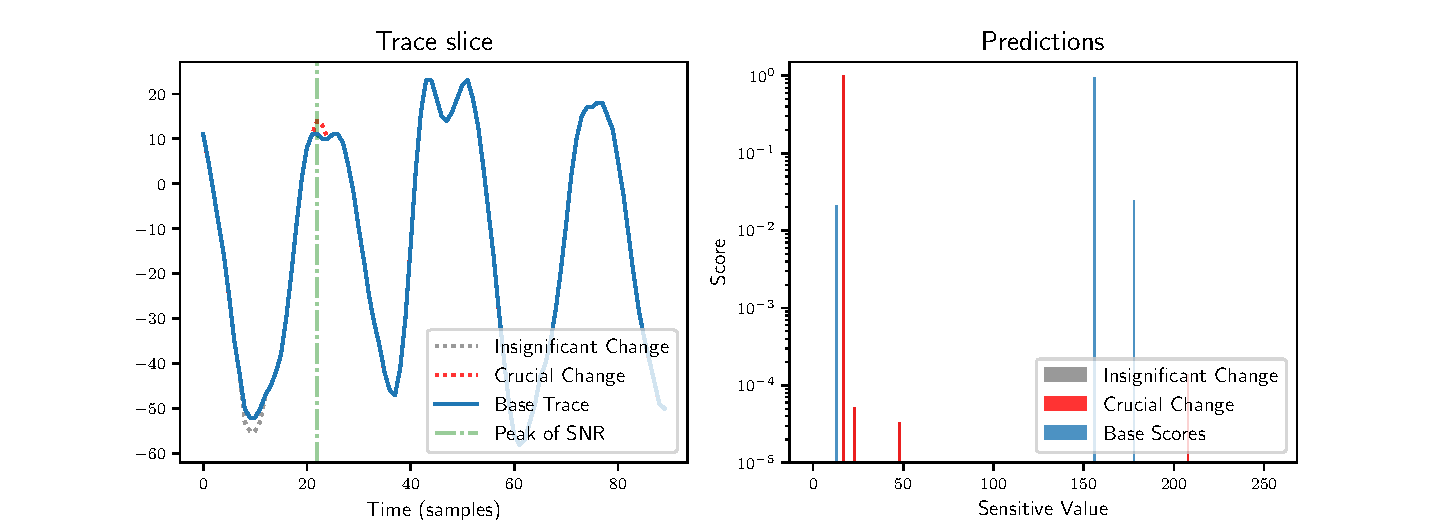
\includegraphics[width=\textwidth]{figures/Illustrations/optimal_model_illustration_review_backup.pdf}
	\caption{Illustration of the Sensitivity Analysis principle. 
	Left: a piece of trace. \(t \in \infoCoord\) is depicted by the green line, and slight variations dotted in red and gray.
	Right: predictions of the optimal model.}
	\label{fig:illustration_cosade}
\end{figure}
Once Assumptions~\ref{assum:sparsity} and~\ref{assum:deriv} are stated, we may want to observe their impact on the properties verified by the optimal model derivatives.
For such a purpose we start by considering an example on a trace \(\xxx\).
\autoref{fig:illustration_cosade} (left) illustrates such a trace in blue, and the green line depicts a \gls{poi}, namely a peak of \gls{snr} -- in other words the set of \glspl{poi} \(\infoCoord\) is reduced to a single time index. 
The \gls{pmf} returned by the optimal model \(\MLmodel^\star(\xxx)\) is given at the right of the same figure: it is here represented by the blue histogram over the 256 possible values of a byte.
We may fairly suppose that a slight variation on one coordinate not belonging to \(\infoCoord\) -- dotted in gray in \autoref{fig:illustration_cosade} (left) -- should not radically change the output of the optimal model. 
The resulting \gls{pmf}, depicted by the gray histogram on \autoref{fig:illustration_cosade} (right) remains the same, as it is perfectly superposed to the blue histogram.
However, applying a slight variation on the coordinate from \(\infoCoord\) -- dotted in red in \autoref{fig:illustration_cosade} (left) -- may radically change the output distribution depicted by the red histogram in \autoref{fig:illustration_cosade} (right).


This example illustrates the more general idea that small variations applied to the trace at a coordinate \(t \in \infoCoord\) should radically change the output prediction whereas small variations at \(t \notin \infoCoord\) should have no impact.
As a consequence, if \(\MLmodel^\star\) is differentiable with respect to the input trace (according to \autoref{assum:deriv}), there should exist \(\sensValue \in \sensVarSet\) such that:
\begin{equation}
	\partDeriv{\xxx[t]} \MLmodel^\star(\xxx)[\sensValue]
	\begin{cases} 
		\neq 0 &\mbox{\gls{iff} } t \in \infoCoord \\
		\approx 0 & \mbox{\gls{iff} } t \notin \infoCoord
	\end{cases}.
\end{equation}
The latter observation can be stated in terms of the \gls{jacob} of the estimator, denoted as \(J_{\MLmodel^\star}(\xxx)\).
Its coefficients should be zero almost everywhere, except in columns \(t \in \infoCoord\):

\begin{equation}
	J_{\MLmodel^\star}(\xxx) = 
	\left(
	\begin{matrix}
		\textbf{0} & \ldots & \textbf{0} & \textbf{Y}_t & \textbf{0} & \ldots & \textbf{0}
	\end{matrix}
	\right) \enspace ,
	\label{eq:jacobian}
\end{equation}
where \(\textbf{Y}_t = \left( \partDeriv{\xxx[t]} \MLmodel^\star(\xxx)[\sensValue_1],
\partDeriv{\xxx[t]} \MLmodel^\star(\xxx)[\sensValue_2], \ldots, \partDeriv{\xxx[t]} \MLmodel^\star(\xxx)\left[\sensValue_{\card{\sensVarSet}}\right] \right)^\intercal\) and 
\(\textbf{0}\) denotes the zero column vector.


The properties verified by the \gls{jacob} matrix in \autoref{eq:jacobian} form the cornerstone of this chapter, as it implies that we can guess from this matrix whether a coordinate from an input trace belongs to \(\infoCoord\) or not, \ie{}, whether a coordinate has been recognized as a \gls{poi} when designing the optimal model \(\MLmodel^\star\).
Moreover, except \autoref{assum:sparsity}, no more assumption on the nature of the leakage model is required.

\section{Proposal for a Characterization Method}
    \label{sec:charac_propal}
    %%%%%%%%%%%%%%%%%%%%%%%%%%%%%%%%%%%%%%%%%%%%%%%%%%%%%%%%%%%%%%%%%%%%%%%%%%%%%%%%
%								CHARAC PROPAL								   %
%%%%%%%%%%%%%%%%%%%%%%%%%%%%%%%%%%%%%%%%%%%%%%%%%%%%%%%%%%%%%%%%%%%%%%%%%%%%%%%%
So far we have shown that the \gls{jacob} of an optimal model \(\jac{\MLmodel^\star}{\xxx}\) may emphasize \glspl{poi}.
In practice however, the evaluator does not have access to the optimal model, but a trained estimation of it, denoted by \(\MLmodel(\cdot, \MLparam)\).
Here we follow this idea in contexts where the approximation is modeled by training \glspl{dnn}.
\autoref{sec:grads_nn} explains how to compute the gradient visualization and the \gls{jacob} based on a trained \gls{dnn}.
\autoref{sec:toy_example} illustrates our claim with a toy example.
Finally, \autoref{sec:related_works} is dedicated to the comparison of our approach with state-of-the-art methods for leakage characterization.


\subsection{Gradient Approximation with Neural Networks}
\label{sec:grads_nn}
In \autoref{sec:universal_approx_thm} we recalled that the universal approximation theorem allows to accurately approximate any function with a \gls{mlp}, up to a precision depending on the number of neurons in the intermediate layers.
It turns out that this theorem also holds for the derivatives of the function to approximate: the latter ones can be accurately approximated by the derivatives of the approximating \gls{mlp}~\cite{hornik_approximation_1991}.%
\footnote{
	The interested reader may refer to the survey of Pinkus~\cite[Sec.~4]{pinkus_approximation_1999}.
}
Hence, the \gls{jacob} of a trained \gls{dnn}, \ie{} \(\jac{\MLmodel(\cdot, \MLparam)}{\xxx}\) represents a sound surrogate to the \gls{jacob} of the optimal model \(\MLmodel^\star\).

To accurately and efficiently compute the \gls{jacob} of a \gls{dnn}, the backprop algorithm presented in \autoref{sec:computing_gradient} can be used.
Originally, it applies a reverse mode differentiation in order to compute the gradient of the loss function with respect to the parameter vector \(\MLparam\).
Interestingly, we explained that the backward pass of the reverse mode actually computes the derivatives of each layer function with respect to each of its inputs, even if the latter ones are not explicitly part of the learning parameters.
This particularly concerns the very first layer which takes as inputs not only some learning parameters but also the input trace \(\xxx\).
In other words, given an input trace \(\xxx\), its corresponding sensitive value \(\z\), and the loss function used for the optimization \(\ell: \probSet{\sensVarSet} \times \sensVarSet \rightarrow \realSet_+\),%
\footnote{
	See a definition in \autoref{eq:loss_function}.
}
it is possible to compute for free the gradient of \(\lossFunc{\MLmodel(\xxx, \MLparam), \z}\) with respect to the input trace \(\xxx\) whenever the gradient of \(\lossFunc{\MLmodel(\xxx, \MLparam), \z}\) with respect to the learning parameters \(\MLparam\) is required.
As a consequence, computing such a gradient can be done with a negligible overhead during an iteration of the \gls{sgd}.

Actually, we justified when presenting the backprop algorithm in \autoref{sec:computing_gradient} that the modern \gls{dl} libraries~\cite{pytorch_2019,tensorflow2015-whitepaper} are optimized to directly compute the gradient of the loss function without explicitly computing the \gls{jacob} \(\jac{\MLmodel(\cdot, \MLparam)}{\xxx}\).
However, our ultimate goal is still to know the \gls{jacob} of the \gls{dnn} model.
Hopefully, studying either the latter one or the gradient of the loss function is fairly equivalent, as one coordinate of the loss function gradient is a function of elements from the corresponding column in the \gls{jacob}, according to \autoref{lemma:chaining_rule}:
\begin{eqnarray}
	\grad[\xxx]{\lossFunc{\MLmodel(\xxx, \MLparam), \sensValue}} & = &
	\jac{\MLmodel(\cdot, \MLparam)}{\xxx}^\intercal \cdot \nabla_{\vNNOutput}\lossFunc{\MLmodel(\xxx, \MLparam),
	\sensValue} \enspace .
\end{eqnarray} 
That is why we propose to visualize the gradient of the loss function, computed with respect to the input trace, to characterize \glspl{poi} in the context of a \gls{dnn} attack, instead of the \gls{jacob} -- unless explicit mention. 
More precisely, we visualize the absolute value of each coordinate of the gradient  in order to get the sensitivity magnitude. 
In the following, such a method is named \glsfirst{gv}.
One of the advantage of this method is that the additional source code required to implement this method is very light, as shown in \autoref{fig:gv_pytorch}.

\begin{figure}
	\centering
	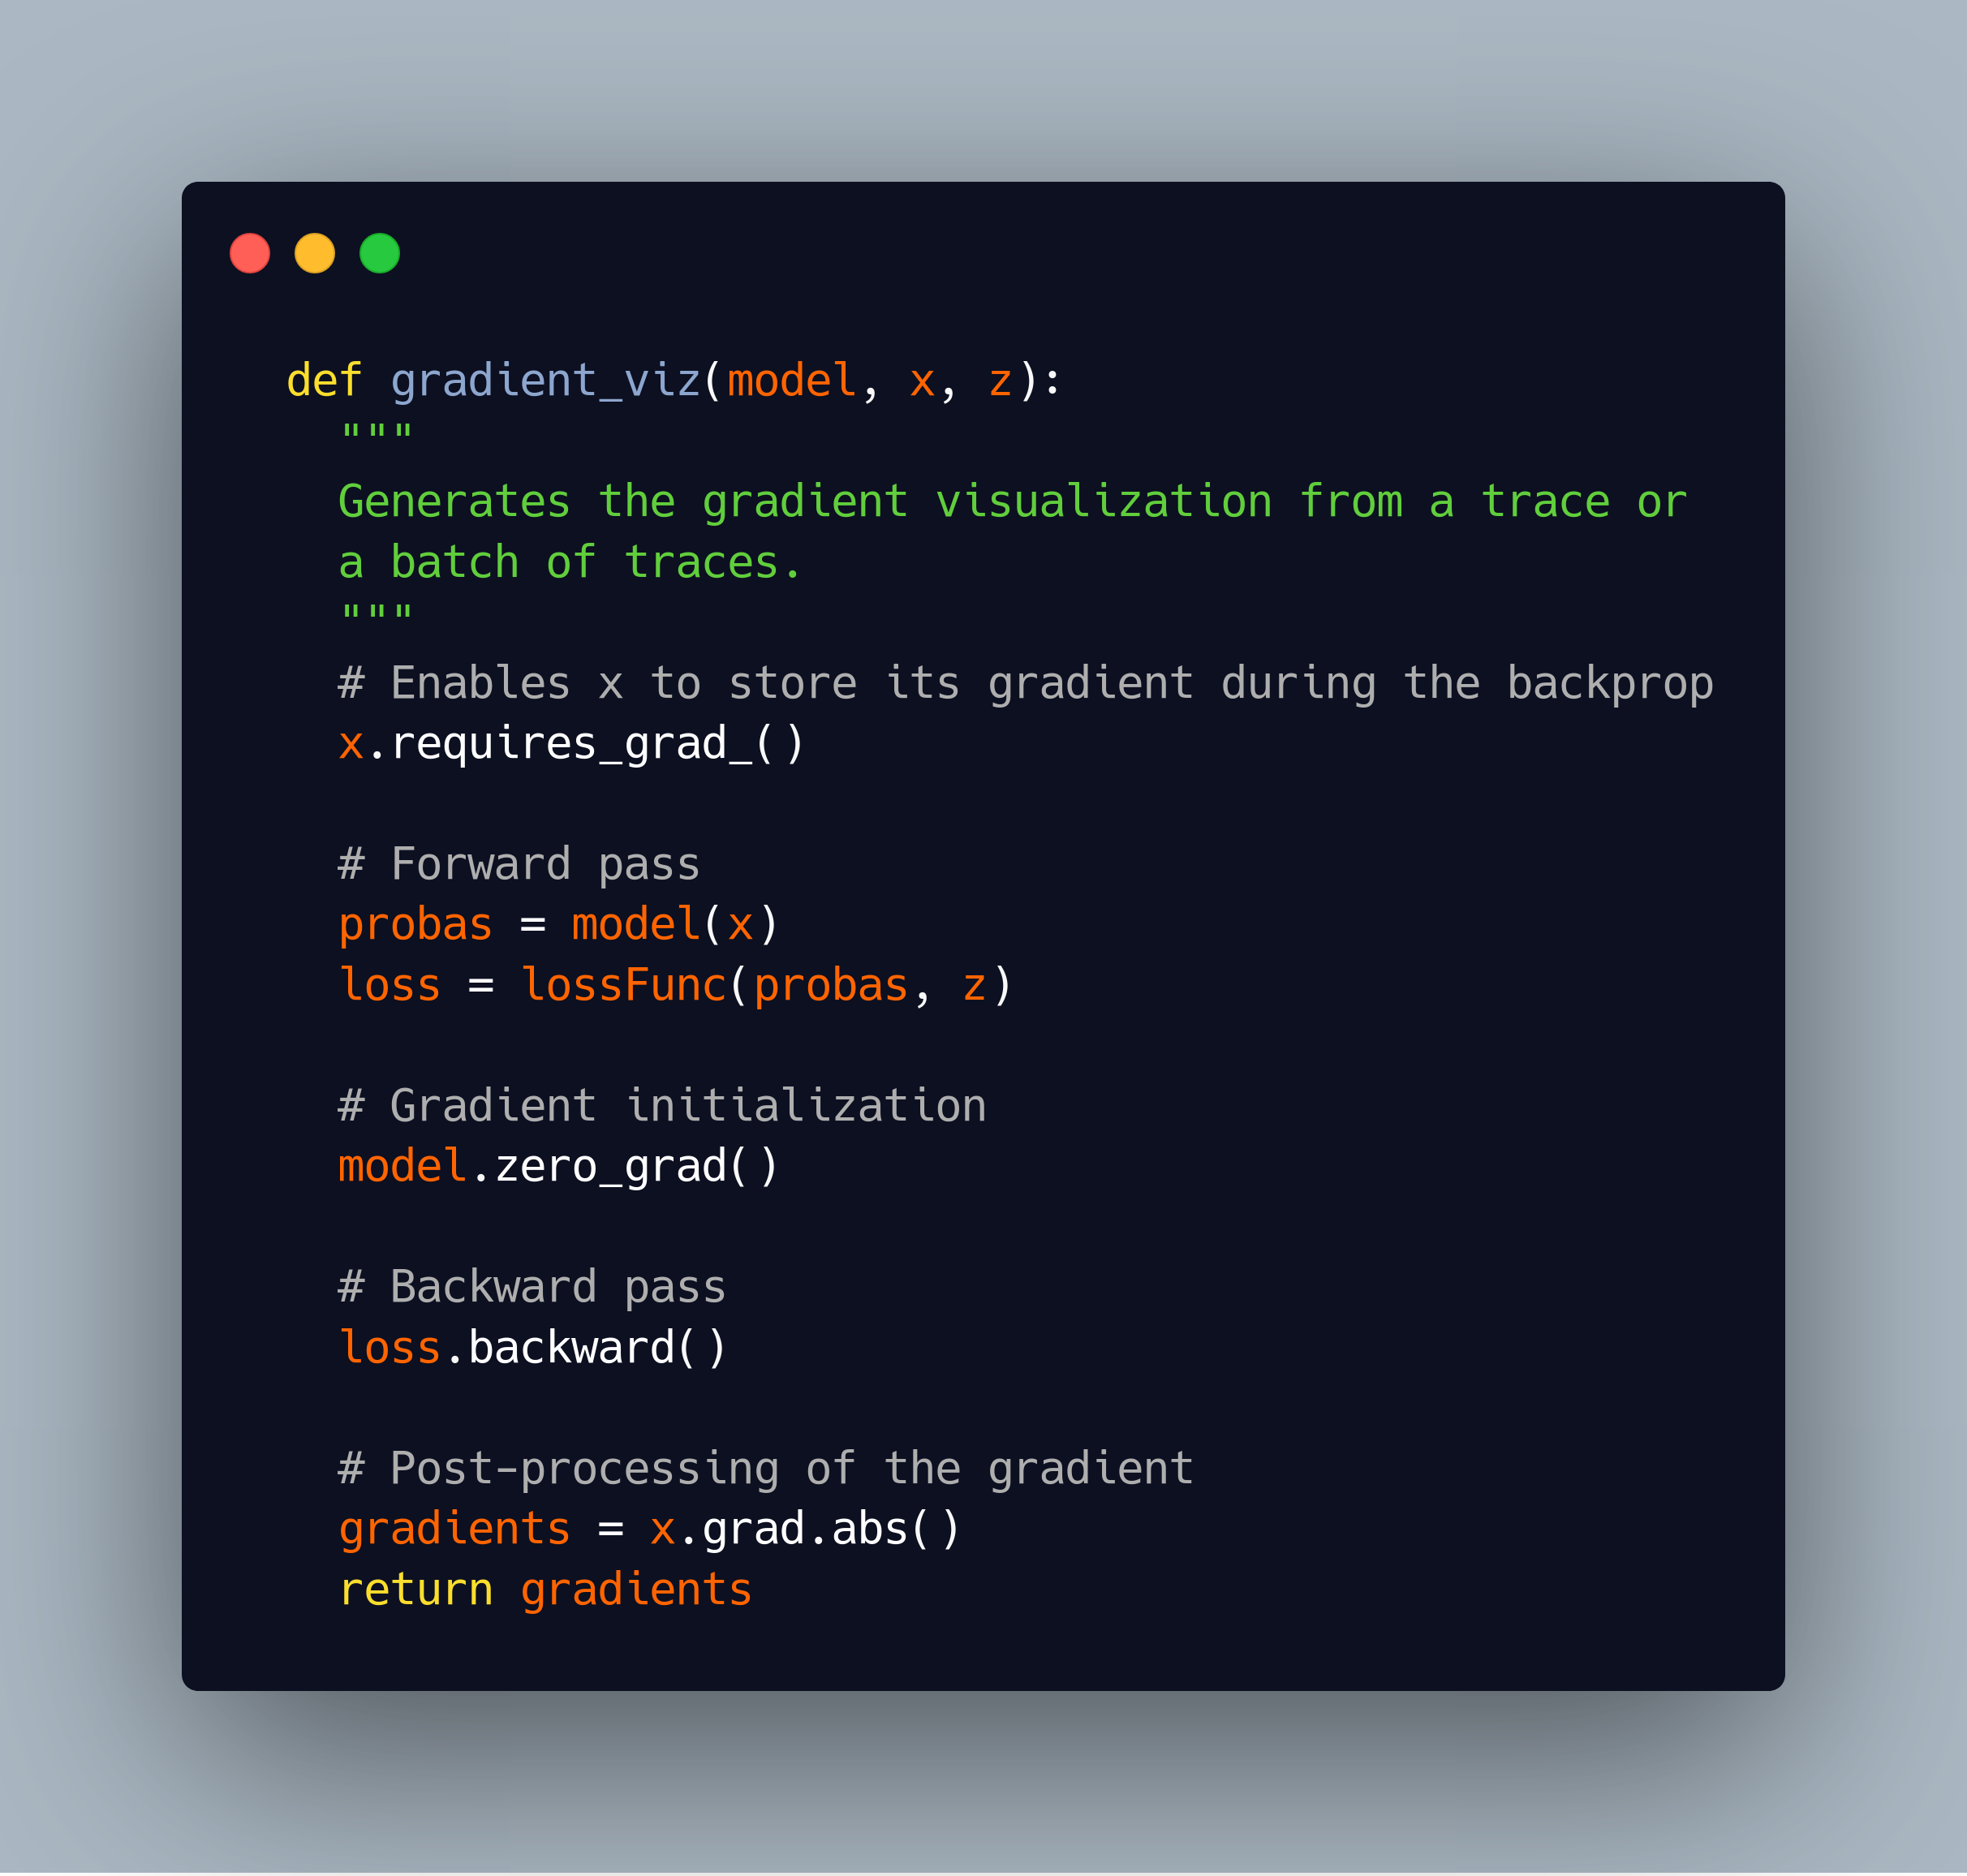
\includegraphics[width = 0.7 \textwidth]{figures/Illustrations/code}
	\caption{Source code to implement the \gls{gv} in \textsf{Pytorch}.}
	\label{fig:gv_pytorch}
\end{figure}

\subsection{Example on Simulated Data}
\label{sec:toy_example}
To illustrate and explain the relevance of the \gls{gv} method, and before going on experimental data, we here propose to apply it on a toy example, aiming at simulating simple \(\traceLength\)-dimensional leakages from an \(n\)-bit sensitive variable \(\Z\).
The method follows the same procedure as already explained in \autoref{sec:settings}.
The traces are defined such that for every \(t \in \llbracket1, \traceLength\rrbracket\):
\begin{equation}
	\xxx_i[t] =
	\begin{cases}
		u_i + b_i \mbox{, if } t \notin \{t_1, \ldots, t_{\order+1}\} \\
		\hWeight(\z_{t,i}) + b_i \mbox{ otherwise}
	\end{cases}
	\enspace ,
\end{equation}
where \((u_i)_i, (b_i)_i\) and all \((\z_{t,i})_i\) are \gls{iid} draws from the following independent random variables.
Respectively, \(\randVar{U} \sim \mathcal{B}(n, 0.5)\), \(\randVar{B} \sim \mathcal{N}(0, \sigma^2)\),%
\footnote{
	It is recalled that \(\hWeight\) denotes the Hamming weight function, see \autoref{sec:cpa}.
} 
where  and where \((\z_{1,i}, \ldots, \z_{\order+1,i})\) is a \((\order+1)\)-sharing of \(\z_i\) for the bit-wise addition law.
This example corresponds to a situation where the leakages on the shares  are hidden among values that have no relation with the target.

Every possible combination of the \(\order\)-sharing has been generated and replicated 100 times before adding the noise, in order to have an exhaustive dataset.
Therefore, it contains \(100 \times 2^{\order n}\) simulated traces. We ran the experiment for \(n = 4\) bits, \(\order \in \{2, 3\}, \traceLength = 100\), and a varying noise \(\sigma^2  \in [0, 1]\). 
Once the data were generated, we trained a neural network with one hidden layer made of \(\traceLength\) neurons.
\begin{figure}
	\centering
	\begin{subfigure}{0.49 \textwidth}
		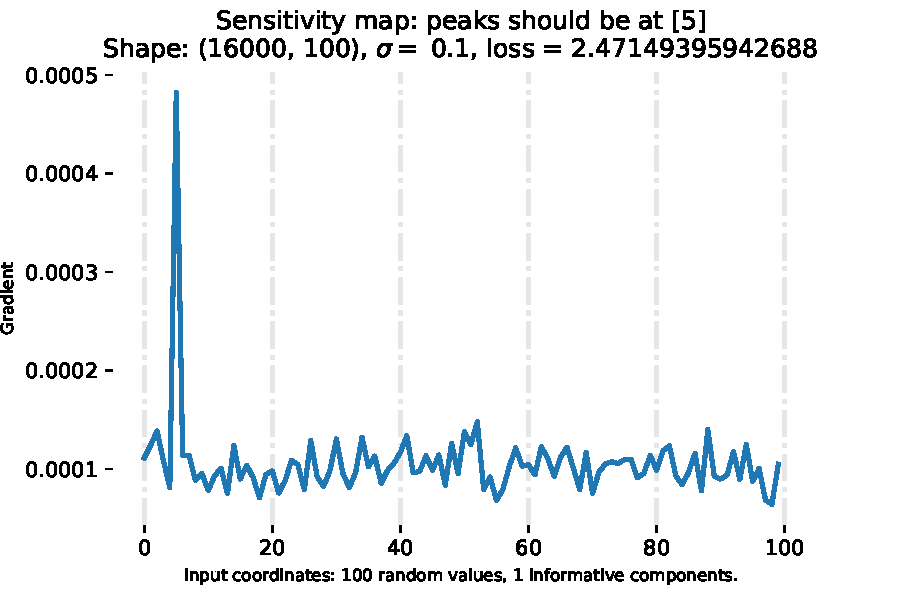
\includegraphics[width=\textwidth]{figures/experience_1/1_shares_shape_16000_100_30_n_hidden_0_dot_1_sigma}
		\caption{One share}
		\label{fig:toy_example_1}
	\end{subfigure}
	\begin{subfigure}{0.49 \textwidth}
		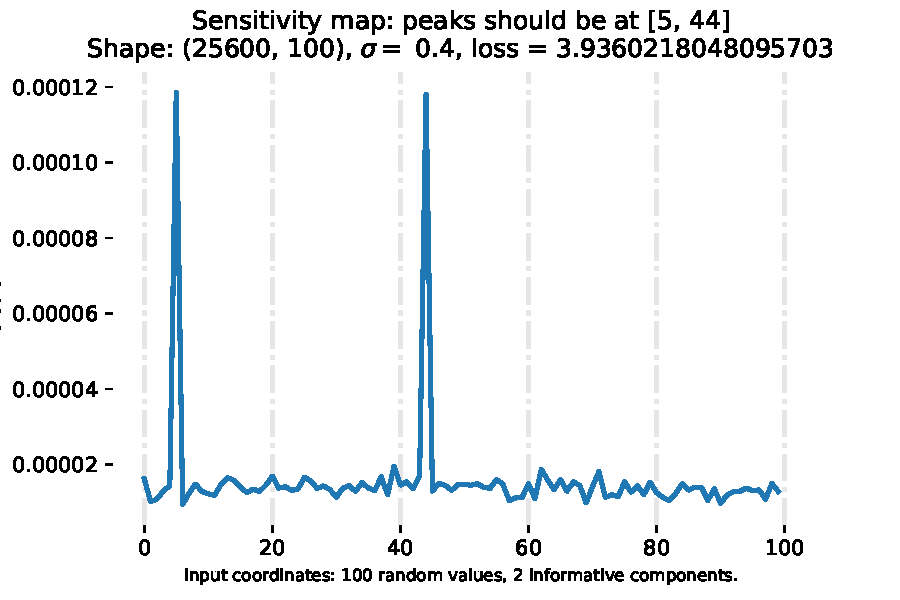
\includegraphics[width=\textwidth]{figures/experience_1/2_shares_shape_25600_100_30_n_hidden_0_4_sigma}
		\caption{Two shares}
		\label{fig:toy_example_2}
	\end{subfigure}
	\begin{subfigure}[]{0.49 \textwidth}
		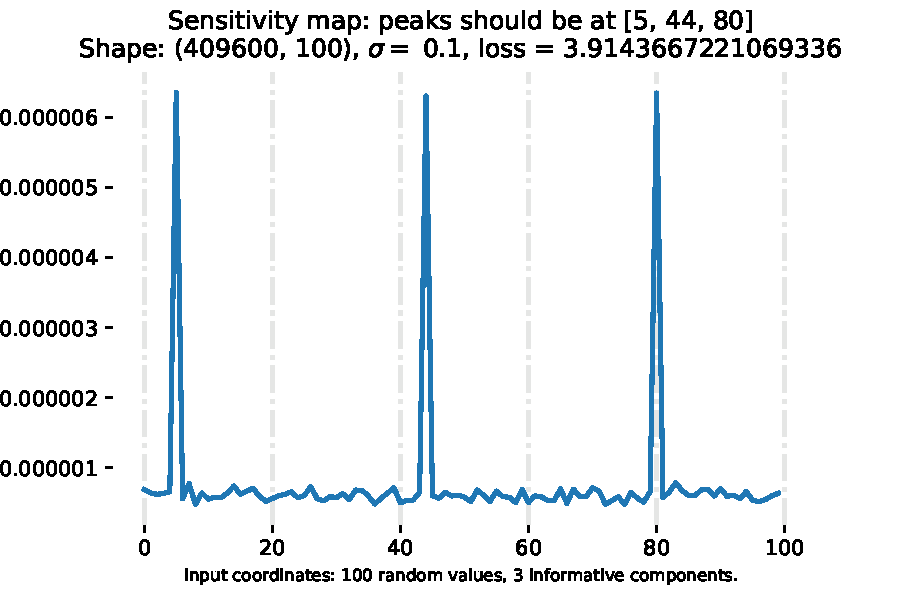
\includegraphics[width=\textwidth]{figures/experience_1/3_shares_shape_409600_100_100_n_hidden_0_1_sigma}
		\caption{Three shares}
		\label{fig:toy_example_3}
	\end{subfigure}
	\caption{Gradient of the loss function, averaged over the validation traces.}
	\label{fig:toy_example}
\end{figure} 
\autoref{fig:toy_example} presents some examples obtained for 1 (\autoref{fig:toy_example_1}), 2 (\autoref{fig:toy_example_2}) and 3 (\autoref{fig:toy_example_3}) shares. 
We clearly see some peaks at the coordinates where the meaningful information have been placed.
This confirms that our characterization method is sound when facing leakages protected by secret-sharing, no matter the order though it required \(16\) times more simulated data and less noised data (\(\sigma^2 \geq 0.1\)) than for the same experiment against first order secret-sharing.


\subsection{Comparison with SNR for Characterization}
\label{sec:related_works}
Now we have shown that \gls{gv} is relevant for characterization on simulated data, one may wonder to what extent this method would be useful compared to other characterization techniques.
In this section, we compare our contribution to the \gls{snr} used for \glspl{poi} selection, as presented in \autoref{sec:characterization}.

One has to keep in mind that the \gls{snr} is a statistical tool, and produces a single characterization from all the profiling traces; whereas our method gives one map for each trace, though we might average them.
This observation has two consequences.
First, if an \gls{snr} characterization is launched in presence of secret-sharing, every trace coordinate \(\XXX[t]\) is likely to be independent from \(\Z\), which will lead the numerator of the \gls{snr} (\autoref{eq:SNR}) to converge towards \(0\).
Secondly, if an \gls{snr} characterization is launched in presence of de-synchronization, then the denominator of \autoref{eq:SNR} is expected to be multiplied by the maximum shift, as argued in \autoref{sec:hiding}.
To sum-up, an \gls{snr} characterization cannot directly highlight higher order leakages when the random material -- used for secret-sharing and/or for de-synchronization -- is not assumed to be known.
Some solutions to deal with this issue have been proposed, \eg{}, by pre-processing the traces with some re-combination functions -- see \autoref{sec:characterization} -- or by applying realignment techniques~\cite{van_woudenberg_improving_2011,nagashima_dpa_2007,durvaux_efficient_2012}.


\subsection{Related Works}
\label{sec:biblio_cosade}
The idea of using the derivatives of differentiable models to visualize information is not new. 
Following the emergence of deep convolutional networks, Simonyan \etal~\cite{simonyan_deep_2013} have first proposed the idea of \gls{gv} to generate a so-called \emph{Sensitivity Map} for image recognition.
The approach was motivated by the fact that such a map can be computed for free thanks to the back-propagation algorithm.
A derived method, called \emph{Guided Backpropagation} has also been proposed by Springenberg \etal{}~\cite{springenberg_striving_2014}.
The latter one slightly modifies the back-propagation rule in a \gls{relu} layer in order to filter the contributions from the upper layers.
Actually, Montavon \etal{}~\cite{montavon_methods_2018} state that visualizing the gradient only tracks an explanation to the variation of a final decision -- \(\MLmodel(\xxx, \MLparam)\) in our context -- and
not directly the decision itself.
To circumvent this, they propose a visualization method called \gls{lrp}.
Another method called \emph{Deconvolution} has been proposed by Zeiler \etal{}~\cite{zeiler_visualizing_2013} in order to give insights about the regions of an input data contributing to the activation of a given feature in a model (either in an intermediate layer or in the output layer).
In the field of Image Recognition, these methods have been shown to be more relevant than \gls{gv}.

However, the \gls{sca} and Image Recognition fields differ.
In the latter one, the decision is highly diluted among lots of pixels, and the decision surface might be locally flat, though we are in an area of interest.
Hopefully in an \gls{sca} context, \autoref{assum:sparsity} states that it is reasonable to consider that the information is very localized.  
That is why we are in a particular case where looking at the output sensitivity may be at least or even more interesting than other visualization methods.

In parallel to the publication of our paper at \textsc{Cosade} 2019, Timon has proposed at \textsc{Ches} 2019 the same method, under the name of sensitivity analysis~\cite{timon_non-profiled_2019}.%
\footnote{
	We prefer using the term ``gradient visualization'' rather than ``sensitivity analysis'' which is a metonymy: the latter one encompasses the former one, beside other techniques.
}
Likewise, Hettwer proposed at \textsc{Sac}'19 a comparison between several techniques such as the \gls{gv}, the \gls{lrp}, and some occlusion techniques~\cite{hettwer_deep_2019}.
The latter ones consist in removing some areas of an input trace, in order to study how a trained model reacts in its predictions.
A relevant area should therefore lead to strong dissimilarities in the corresponding predictions when it is removed.
Later, Zaid \etal{} proposed the use of \emph{heatmaps}~\cite{zaid_methodology_2019}.%
\footnote{Another technique used by the authors, called \emph{weight visualization} is rather focused on the understanding of the learned weights of the dense layers in a \gls{cnn}, therefore beyond the scope of this study.}
It consists in computing the average output over all filters of a given convolution layer.
In particular, the heatmap of the first layer is expected to produce a similar map as the \gls{gv}.
Wouters \etal{}, in a paper revisiting the results of Zaid \etal{}, used a variant of the \gls{gv} called \emph{Gradient \(\times\) Input} consisting in multiplying the map returned by \gls{gv} with the input trace itself~\cite{wouters_revisiting_2020}.
Likewise, Van der Valk \etal{} have investigated the \emph{Singular Vector Canonical Correlation Analysis} provide insights on the layers of a trained \gls{mlp}~\cite{vanDerValk_kilroy_2019}.
Finally, Bursztein \etal{} presented at \textsc{Defcon} 2020 a tool involving explainability techniques for \gls{dl} similar to \gls{gv}~\cite{elie_scadl_2020}.
By using characterization maps similar to the ones produced by the \gls{gv} method, they are able to produce a mapping with the assembly instructions yielding the informative leakage.
Thanks to a reverse-engineering tool, they are able to map the leaky assembly instructions to the corresponding area in the code, enabling to precisely identify the vulnerability.

\section{Experimental Verification}
    \label{sec:method_cosade}
    %%%%%%%%%%%%%%%%%%%%%%%%%%%%%%%%%%%%%%%%%%%%%%%%%%%%%%%%%%%%%%%%%%%%%%%%%%%%%%%%
%                               MÉTHODE CHAPTER 7	                           %
%%%%%%%%%%%%%%%%%%%%%%%%%%%%%%%%%%%%%%%%%%%%%%%%%%%%%%%%%%%%%%%%%%%%%%%%%%%%%%%%
So far we have claimed that relevant information can be extracted from the loss gradient of a differentiable model.
Following this idea, it has been shown to be efficient to localize \glspl{poi} on simulated data and we validated that this method might overcome some weaknesses of state-of-the-art techniques.
We now plan to experimentally verify these claims on three experimental datasets.

We first conduct comprehensive experimentations on the \gls{ascad} datasets.
Before introducing the results in \autoref{sec:exp_res_cosade}, we first describe our investigations.
In \autoref{sec:cnn_archi_cosade}, we present the \gls{cnn} architecture used for profiling, and \autoref{sec:settings_cosade} gives an exhaustive description of all the considered parameters for our experiments.

Then, we also verify the soundness of the \gls{gv} method over the two polymorphism datasets.
The results are reported in \autoref{sec:gv_claps}.

\subsection{CNN Architecture}
\label{sec:cnn_archi_cosade}
For these experiments, we consider a \gls{vgg}-based architecture, that we recall hereafter:
\begin{equation}\label{eq:vgg_archi_cosade}
	\MLmodel = 
	\softmax \circ \linLayer_{\card{\sensVarSet}} \circ [\actLayer \circ \linLayer_\linSize]^{n_1}
	\circ [\poolLayer_\pstride \circ \actLayer \circ \BNLayer \circ \convLayer_{\ksize, \numFilters}]^{n_2} \circ \BNLayer \enspace ,
\end{equation}
where \(\convLayer_{\ksize, \numFilters}\) denotes a convolutional layer made of \(\numFilters\) filters of size \(\ksize\), \(\BNLayer\) denotes a batch-normalization layer, \(\actLayer\) denotes the \gls{relu} activation function, \(\poolLayer_{\pstride}\) denotes an average pooling layer of size \(\pstride\), \(\linLayer_{\linSize}\) denotes a dense layer, and \(\softmax\) denotes the softmax layer.
Furthermore, the composition \([\poolLayer_{\pstride} \circ \actLayer \circ \BNLayer \circ \convLayer_{\ksize, \numFilters}]\) is denoted as a convolutional \emph{block}.
Likewise, \([\actLayer \circ \linLayer]\) denotes a dense block.
We note \(n_1\) (resp. \(n_2\)) the number of dense blocks (resp. convolutional blocks).
The details of this architecture have been presented in \autoref{sec:pres_architectures}.
We chose this architecture since it is the baseline used in the works of Benadjila \etal{}~\cite{prouff_study_2018} introducing the \gls{ascad} database on which we work -- see \autoref{sec:ascad}.

As the ultimate goal is not to get the best architecture as possible, but rather having a simple and efficient one, a lighter baseline has been chosen compared to the original architecture proposed in the authors' work: 
\begin{itemize}
	\item The number of filters in the first layers has been decreased, \ie{}, \(\numFilters_0 = 10\) instead of 64, though it is still doubled between each block: 
	\begin{equation}
		\numFilters_i = \max(512, \numFilters_0 \times 2^i) \enspace ,
	\end{equation}
	where \(\numFilters_n\) denotes the number of filters at the \(i\)-th convolutional block for \(i \leq n_2\) and the filter size has been set to \(\ksize=5\).
	\item The dense layers contain less neurons: \(\linSize = 1,000\) instead of 4,096.
	\item The last pooling layer is global -- see \autoref{sec:cnn_archi_esorics} -- \ie{}, its pooling size equals the width of the feature maps in the last convolutional layer, so that each feature maps are reduced to one point.
	While it drastically reduces the number of neurons in the first dense layer and thereby its number of weights to learn, the global pooling layer also forces the convolutional filters to better localize the discriminative features~\cite{zhou_learning_2016}.
\end{itemize}

\subsection{Settings of the Experiments}
\label{sec:settings_cosade}
Our experiments have been done with the \(50,000\) \gls{em} traces from the \gls{ascad} database, presented in \autoref{sec:ascad}.
Each trace is made of \(700\) time samples.%
\footnote{
	It corresponds to 26 clock cycles.
}
Hereafter, the three different configurations investigated in this chapter are presented with the notations taken from \cite{prouff_study_2018}. 
For each experiment we precise the label to be learned.
This label is known during the profiling phase but not during the attack phase:
\begin{itemize}
	\item \textbf{Experiment 1 (no counter-measure)}: the traces are synchronized, the label to learn is \(\Z = \Sbox(\Pt \plusgf \keyTest) \plusgf \rout\), where \(\rout\) is a random share used to protect the leakage of the \(\Sbox\) output -- see \autoref{sec:ascad}.
	In other terms, \(\rout\) is assumed here to be known, like \(\Pt\).
	The traces correspond to the dataset \verb+ASCAD.h5+, and the labels are recomputed from the \verb+metadata+ field of the \verb+hdf5+ structure.
    \item \textbf{Experiment 2 (artificial shift)} : the labels are the same as in Exp.~1 but the traces are  artificially shifted to the left of a random number of points drawn from a uniform distribution over \(\llbracket0, 100\rrbracket\).
    The traces correspond to the dataset \verb+ASCAD_desync100.h5+.
	\item \textbf{Experiment 3 (synchronized traces, with secret-sharing)}: we target \(\Z = \Sbox(\Pt \oplus \keyTest)\), \ie{}, we have no knowledge anymore of the random share \(\rout\) -- neither during profiling or attack phase. Concretely, the traces correspond to the dataset \verb+ASCAD.h5+ and the labels are directly imported from the field \verb+labels+ in the \textsf{hdf5} structure.
\end{itemize}
It is noticeable that in every case, as the key is fixed, and both the plaintext and the share \(\rout\) are completely random and independent.
Therefore, the labels are always balanced.

Following the results presented in \autoref{chap:ches_20}, we use the \gls{nll} as a loss function.
The settings have been made so that any experiment is reproducible: random seeds are known, and all the settings of the \gls{gpu} are set to avoid stochastic behavior.%
\footnote{Usually, forcing the \gls{gpu} to have a fully deterministic behavior implies worse runtime performance.}
For each tested neural network architecture, a \(5\)-fold \emph{cross-validation} strategy has been followed. Namely, the \gls{ascad} database has been split into \(5\) sets \(\mset{S}_1, \ldots, \mset{S}_5\) of \(10,000\) traces each, and the \(i\)-th cross-validation, denoted by \(\mathrm{CV}_i\), corresponds to a training dataset \(\trainSet=\cup_{j\neq i} \mset{S}_j\) and a validation dataset \(\valSet = \mset{S}_i\).
The given performance metrics and the visualizations are averaged over these 5 folds. 
The optimization is done with the \gls{adam} algorithm -- see \autoref{sec:optim_algo}.
The learning rate is always set to \(10^{-4}\).
Likewise, the batch size has been fixed to \(64\).
For each training, we operate 100 epochs, \ie{} each couple \((\xxx_i, \z_i)\) is passed 100 times through an iteration of the optimization algorithm, and we keep as the best model the one that has the lowest \gls{ge} on the validation set.%
\footnote{
	Following the discussion in \autoref{chap:ches_20}, the other \gls{ml} metrics are ignored.
}

\section{Results}
    \label{sec:exp_res_cosade}
    %%%%%%%%%%%%%%%%%%%%%%%%%%%%%%%%%%%%%%%%%%%%%%%%%%%%%%%%%%%%%%%%%%%%%%%%%%%%%%%%
%                           RESULTS EXPERIMENTS CHAPTER 7                      %
%%%%%%%%%%%%%%%%%%%%%%%%%%%%%%%%%%%%%%%%%%%%%%%%%%%%%%%%%%%%%%%%%%%%%%%%%%%%%%%%
This section presents experimentations of the \gls{gv} in different contexts, namely (Exp.~1) when the implementation embeds no counter-measure, (Exp.~2) when traces are de-synchronized and (Exp.~3) when Boolean secret-sharing is applied.
The methods used to train the \glspl{cnn}, to tune their \glspl{hp} and to generate the \gls{gv} have been presented in \autoref{sec:method_cosade}.

\subsection{Application Without Counter-measure}
\label{sec:no_mask_no_desynchro}

\begin{table}
    \centering
    \caption{Settings and results of Exp.~1}
	\label{table:no_mask_no_desync}
    \begin{subtable}{0.49 \textwidth}
        \centering
        \caption{Architecture \glspl{hp}.}
        \begin{tabular}{l r}
            \toprule
            Parameter & Value \\
            \midrule
            \(n_2\) & 5 \\
            \(n_1\) & \{0, 1, 2\} \\
            \bottomrule
        \end{tabular}
        \label{table:no_mask_no_desync_left}
    \end{subtable}
    \begin{subtable}{0.49 \textwidth}
        \centering
        \caption{Performance metrics without counter-measure.}
        \begin{tabular}{l c r}
            \toprule
            \(n_1\) & Loss (bit) & \(\numTracesAttack(\MLmodel)\) \\
            \midrule
            0 & \(6.40\) & \(3.25\) \\
            1 & \(6.15\) & \(3\) \\
            2 & \(6.35\) & \(3.25\) \\
            \bottomrule
        \end{tabular}
        \label{table:no_mask_no_desync_center}
    \end{subtable}
\end{table}

In application context (Exp.~1) -- \ie{} no counter-measure -- several \glspl{cnn} have been trained with the architecture \glspl{hp} in \autoref{eq:vgg_archi_cosade} specified as listed in \autoref{table:no_mask_no_desync_left}. 
Since the random shares are here directly targeted -- \ie{} the masks are supposed to be known -- without re-combination -- thereby no dense layer -- should be required, according to the study of Benadjila \etal{}~\cite[Sec.~4.2.4]{prouff_study_2018}. 
The \gls{hp} \(n_1\) should therefore be null. 
However, to validate this intuition we let it vary in \(\{0,1,2\}\). 
The validation loss corresponding to these values is given in \autoref{table:no_mask_no_desync_center}, where \(\numTracesAttack(\MLmodel)\) denotes here the minimum number of traces required to have a \gls{ge} lower than \(1\).
Even if this minimum is roughly the same for the three different configurations, we selected the \emph{best} one 
-- \ie{} \(n_1=1\) -- for our \emph{best} \gls{cnn}  architecture. 
\autoref{fig:no_mask_no_desynchro_gv} presents the corresponding \gls{gv}, and \autoref{fig:no_mask_no_desynchro_snr} depicts the corresponding \gls{snr}.
It may be observed that the peaks obtained with \gls{gv} and \gls{snr} are identical: the highest point in the \gls{snr} is the second highest point in \gls{gv}, whereas the highest point in \gls{gv} is ranked \(7\)-th in the \gls{snr} peaks. 
More generally both methods target the same clock cycle (the \(19\)-th).
These observations validate the fact that our characterization method is relevant for an unprotected target.

\begin{figure}
    \centering
    \begin{subfigure}{0.49 \textwidth}
        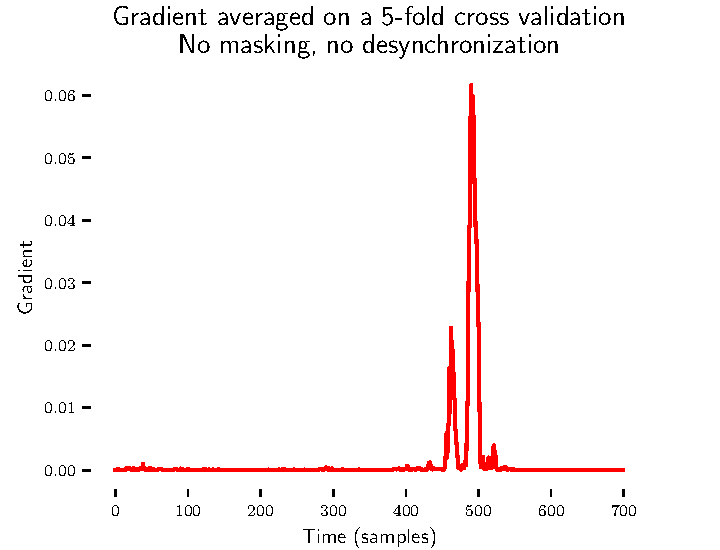
\includegraphics[width=\textwidth]{figures/ASCAD_700/no_mask_no_desynchro/VBP_n_dense_1_mean_review}
        \caption{\gls{gv} for the trained model with one dense layer, averaged over the validation traces.}
        \label{fig:no_mask_no_desynchro_gv}
    \end{subfigure}
    \begin{subfigure}{0.49 \textwidth}
        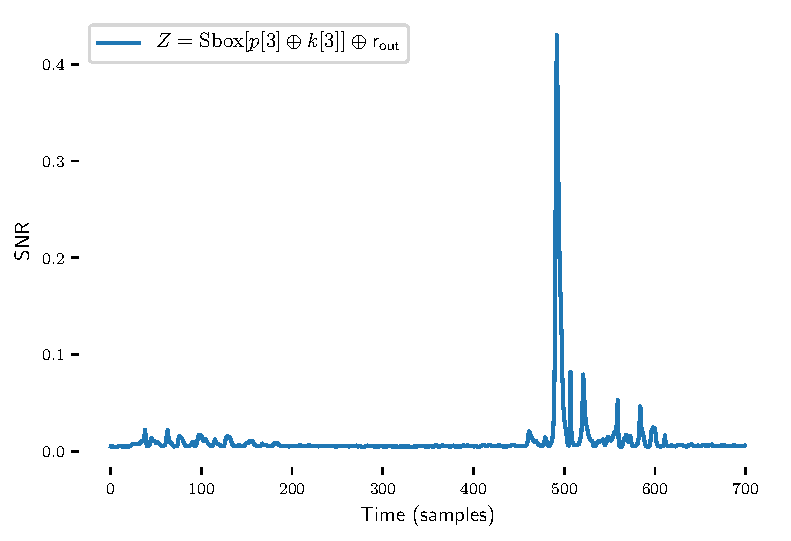
\includegraphics[width=\textwidth]{figures/ASCAD_700/snr_ascad_unmasked}
        \caption{The corresponding \gls{snr}.}
        \label{fig:no_mask_no_desynchro_snr}
    \end{subfigure}
	\caption{Case where no counter-measure is considered.}
    \label{fig:no_mask_no_desynchro}
\end{figure}
In addition to the \gls{gv} we also show in \autoref{fig:jacob_exp_1} the \gls{jacob} of the trained model.
Around the time coordinate 500 along the x-axis, some blue areas depict a high value in the matrix.
One may remark that those blue areas particularly appear for value of the sensitive variable -- along the  ordinates axis -- whose Hamming weight is one.
Since a high value in the \gls{jacob} implies a high sensitivity to slight changes in the input trace at the considered time coordinate, we may imagine that the trained \gls{cnn} is able to give a high confidence when expected to predict those values of the sensitive variable.
In other words, they are more distinguishable than the other values.
Although not a formal proof, this observation is coherent with a Hamming weight leakage model, where values of the target variable with low -- \eg{} 0 or 1 -- or high -- \eg{} 7 or 8 -- Hamming weight are more distinguishable than the others.
This example hence shows how the \gls{jacob} can bring additional insights compared to the gradient.

\begin{figure}[h]
    \centering
    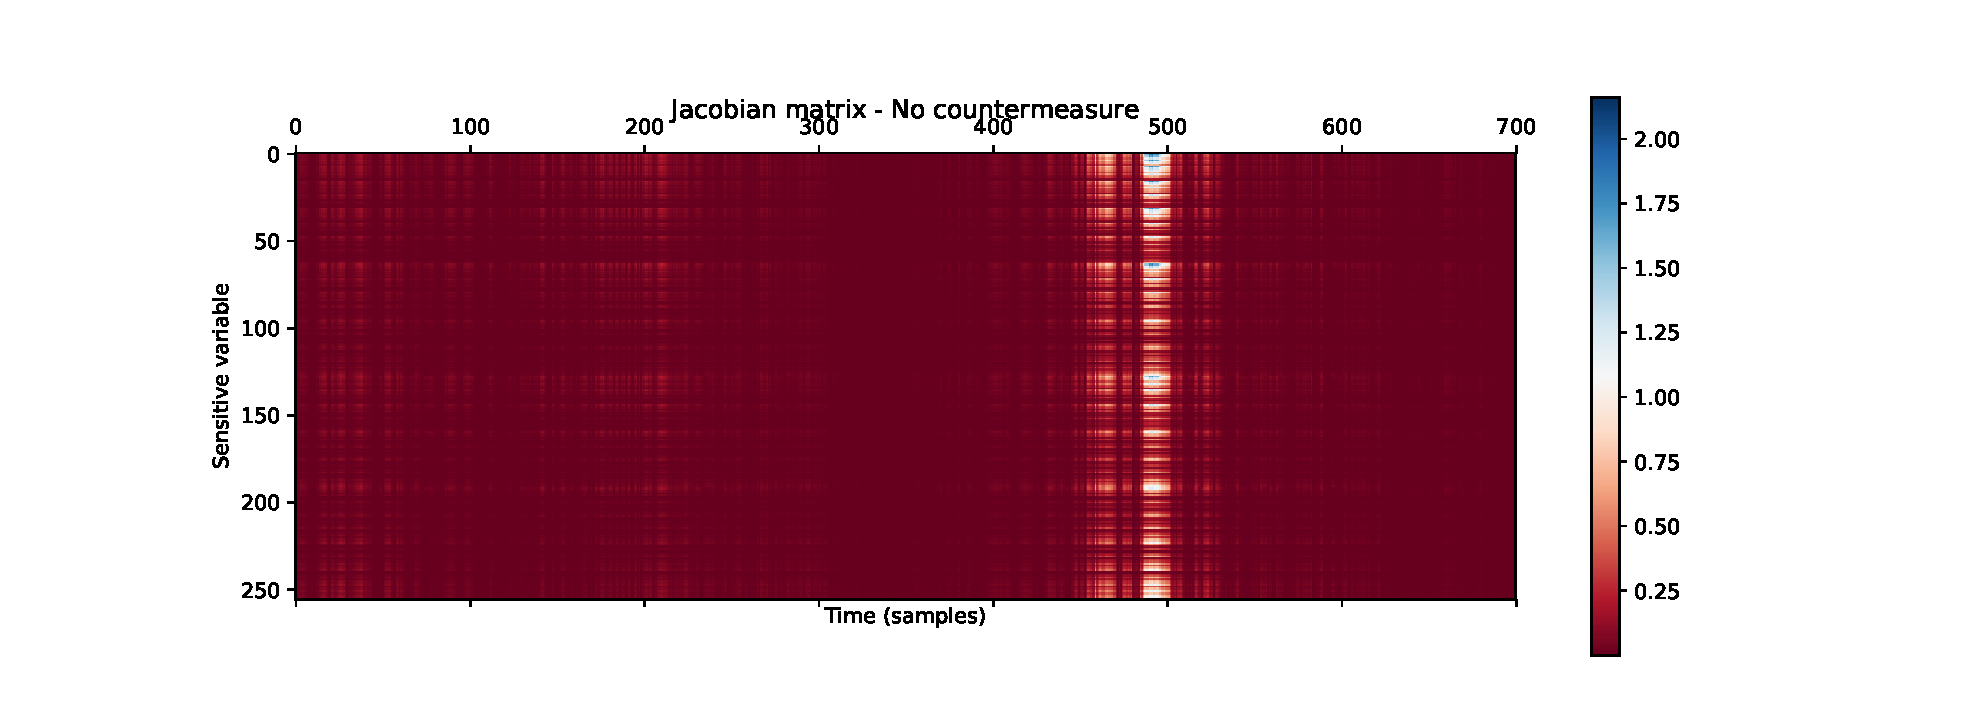
\includegraphics[width=\textwidth]{figures/ASCAD_700/no_mask_no_desynchro/jacob_n_dense_0_CV_0}
    \caption{\gls{jacob} for the best models in application context Exp.~1.}
    \label{fig:jacob_exp_1}
\end{figure}

\subsection{Application with an Artificial De-synchronization}
\label{sec:no_mask_with_desynchro}
\begin{table}
    \centering
    \caption{Settings and results of Exp.~2}
    \label{table:no_mask_with_desync}
    \begin{subtable}{0.49 \textwidth}
        \centering
        \caption{Architecture \glspl{hp}.}
        \begin{tabular}{l r}
            \toprule
            Parameter & Value \\
            \midrule
            \(n_2\) & 5 \\
            \(n_1\) & \{0, 1, 2\} \\
            \bottomrule
        \end{tabular}
        \label{table:no_mask_with_desync_left}
    \end{subtable}
    \begin{subtable}{0.49 \textwidth}
        \centering
        \caption{Performance metrics with de-synchronization.}
        \begin{tabular}{l c r}
            \toprule
            \(n_1\) & Loss (bit) & \(\numTracesAttack(\MLmodel)\) \\
            \midrule
            0 & \(6.64\) & \(4.0\) \\
            1 & \(6.46\) & \(3.6\) \\
            2 & \(6.90\) & \(5.4\) \\
            \bottomrule
        \end{tabular}
        \label{table:no_mask_with_desync_right}
    \end{subtable}
\end{table}

We now add a new difficulty by considering the case of de-synchronization as described in \autoref{sec:settings_cosade}.
The \gls{hp} grid is exactly the same as in \autoref{sec:no_mask_no_desynchro}, and the corresponding loss is given in \autoref{table:no_mask_with_desync_right}. 
Faced to misalignment, the considered architectures have still good performances, and the attacks succeeded in roughly the same number of traces than before. 
Interestingly, \autoref{fig:no_mask_with_desynchro} shows that the \gls{gv} succeeds in recovering the leakage localization while the \gls{snr} does not. 
Actually, the gradient averaged over the profiling traces \autoref{fig:no_mask_with_desynchro_gv_avg} shows that, instead of having a small number of peaks, a band is obtained whose width approximately equals the maximum quantity of shift applied in the traces, namely 100 points. 
Moreover, individual gradients in \autoref{fig:no_mask_with_desynchro_gv_single} bring a single characterization for each trace, enabling to guess approximately the shift applied to each trace.

\begin{figure}
    \centering
    \begin{subfigure}[]{0.49 \textwidth}
        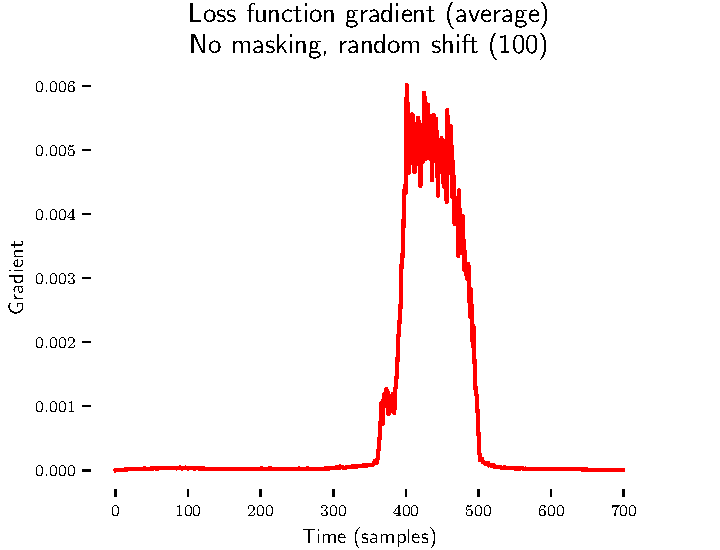
\includegraphics[width=\textwidth]{figures/ASCAD_700/no_mask_with_desynchro/grads_avg_n_dense_1_review}
        \caption{\gls{gv} averaged over all the traces.}
        \label{fig:no_mask_with_desynchro_gv_avg}
    \end{subfigure}
	\begin{subfigure}[]{0.49 \textwidth}
        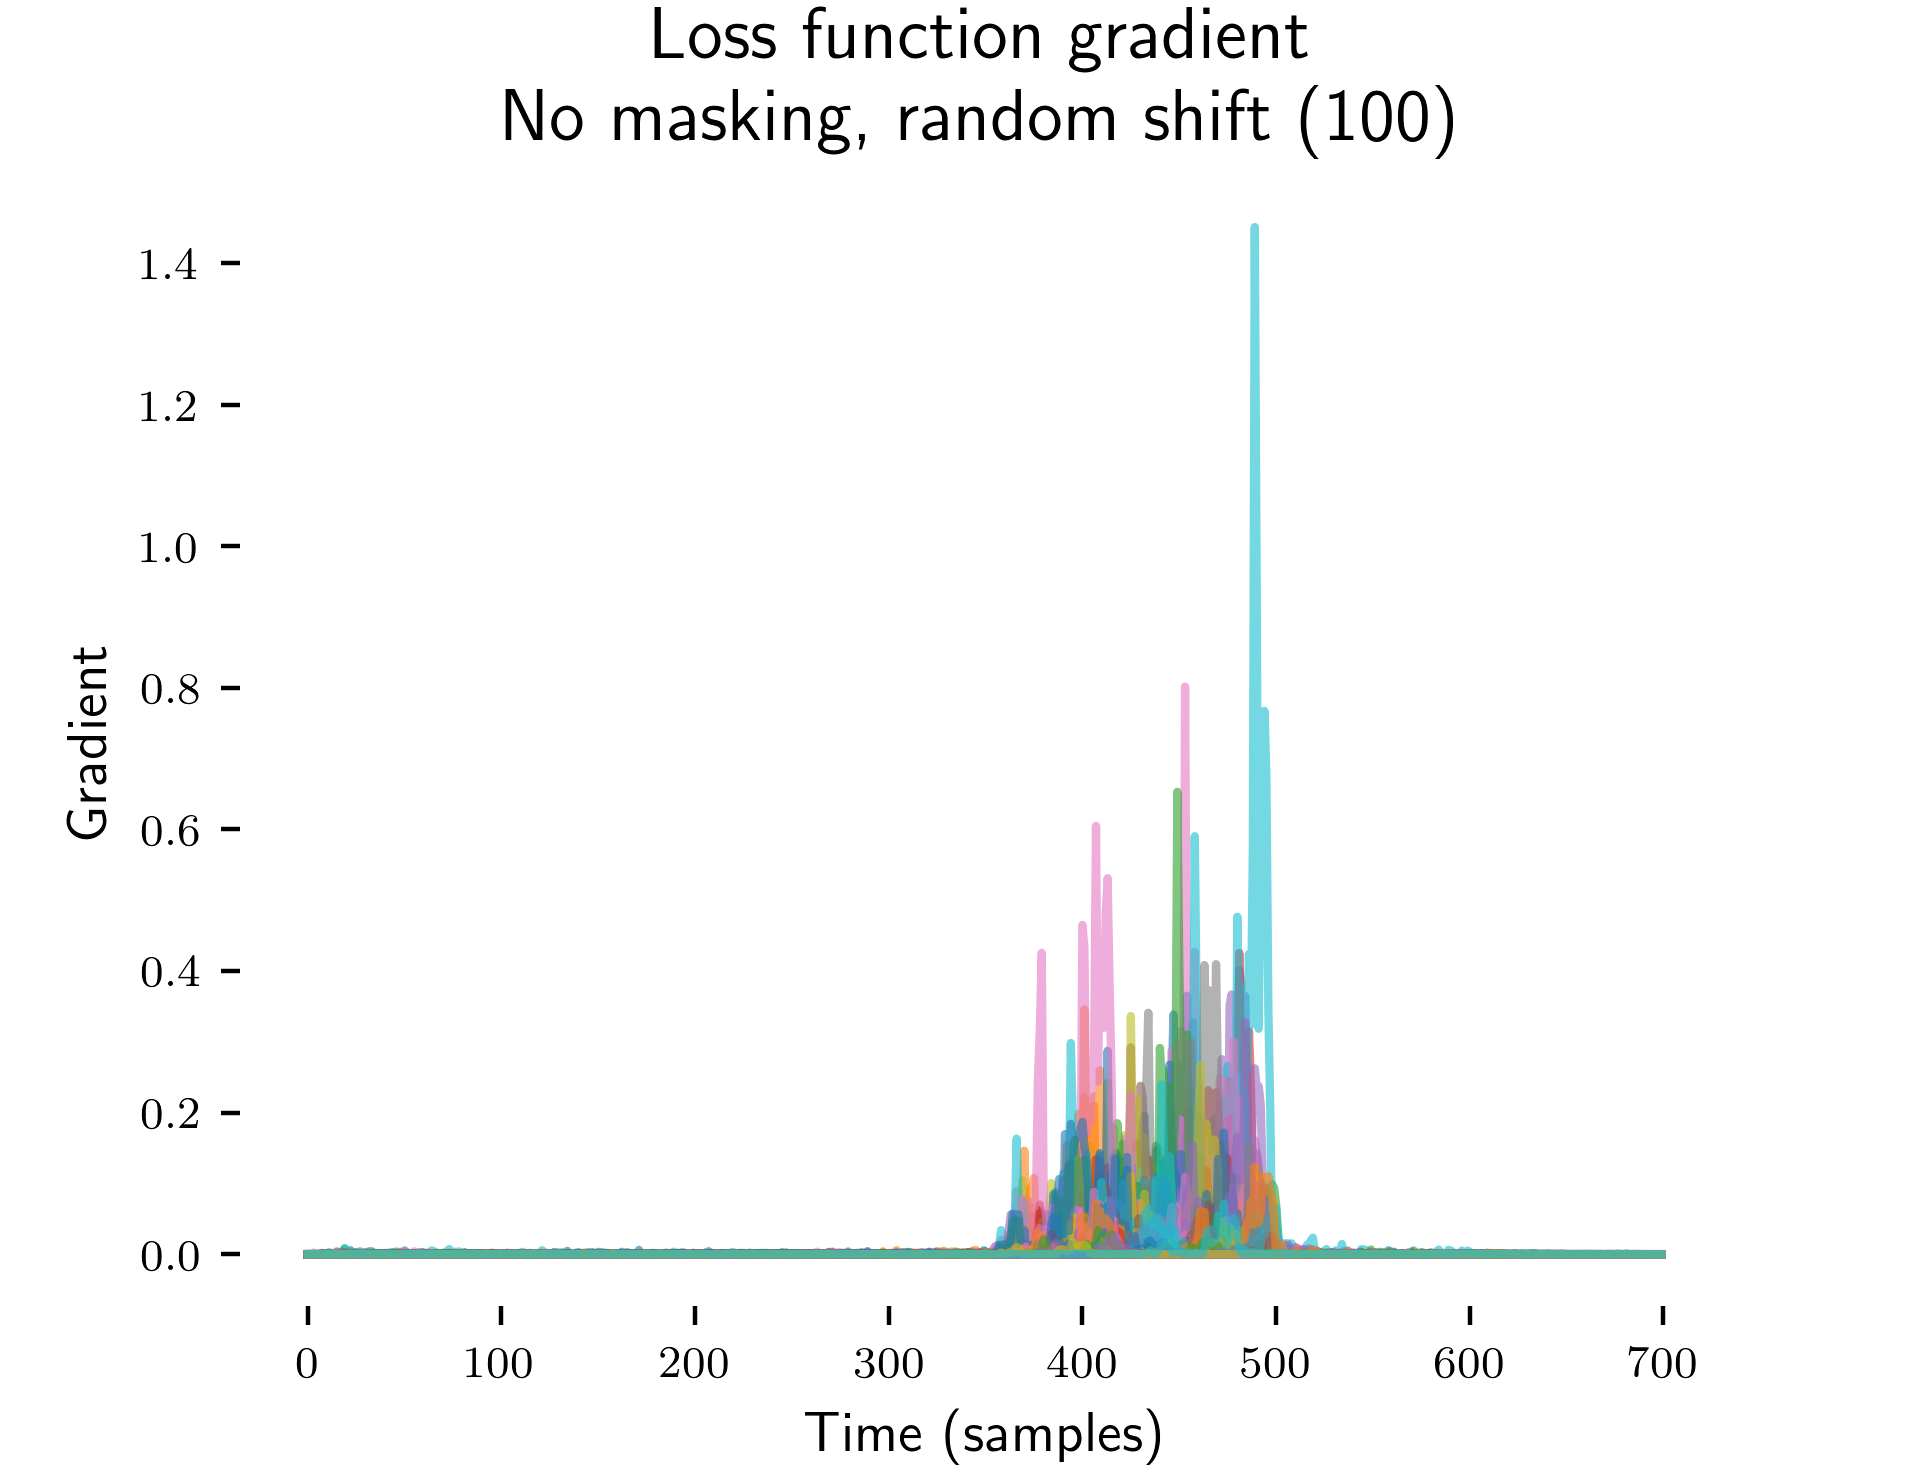
\includegraphics[width=\textwidth]{figures/ASCAD_700/no_mask_with_desynchro/all_grads_review.png}
        \caption{\gls{gv} for each trace separately.}
        \label{fig:no_mask_with_desynchro_gv_single}
    \end{subfigure}
    \begin{subfigure}[]{0.49 \textwidth}
        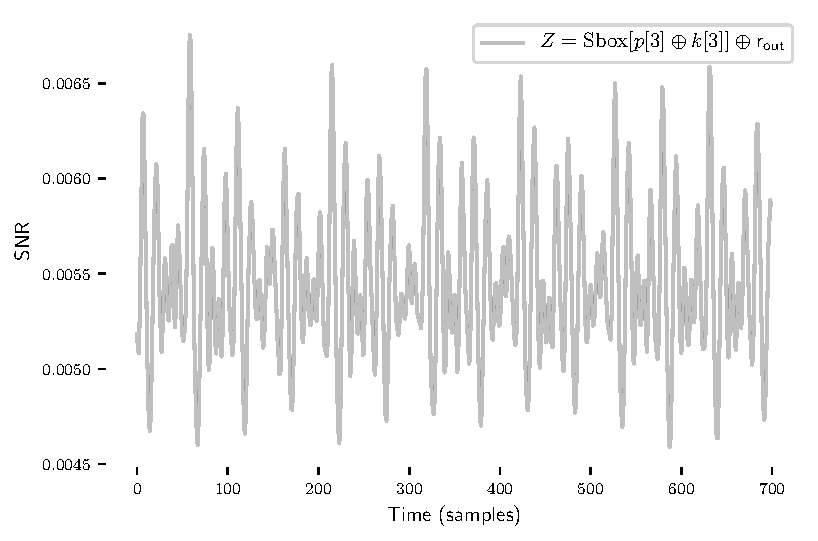
\includegraphics[width=\textwidth]{figures/ASCAD_700/snr_desync100}
        \caption{The corresponding \gls{snr}.}
        \label{fig:no_mask_with_desynchro_snr}
    \end{subfigure}
	\caption{Case where de-synchronization is considered.}
	\label{fig:no_mask_with_desynchro}
\end{figure}

\subsection{Application with a First Order Secret-Sharing}
\label{sec:with_mask_no_desynchro}
The next experiment concerns the application of \gls{gv} in presence of Boolean secret-sharing, namely the one implemented in the \gls{ascad} dataset.
Several model configurations have been tested which correspond to the \glspl{hp} listed in \autoref{table:ge_masking_hp}.
We eventually selected the \(8\) models that achieved the best efficiency, \ie{} the model \(\MLmodel(\cdot, \MLparam)\) with the lowest \(\numTracesAttack(\MLmodel)\) (\autoref{table:ge_masking_perf}).%
\footnote{
    Contrary to the convention taken in \autoref{sec:performance_metrics}, \(\numTracesAttack(\MLmodel)\) is here computed with respect to the \gls{ge}, as defined by \autoref{eq:eff_ge}.
}
 
\begin{table}
    \begin{subtable}{.49\textwidth}
        \centering
        \caption{Architecture \glspl{hp} -- bold values refer to the best choices.}
        \label{table:ge_masking_hp}
        \begin{tabular}{l r}
            \toprule
            Parameter & Value \\
            \midrule
            \(n_2\) & \{5, 6, \textbf{7}, 8\} \\
            \(n_1\) & \{\textbf{2}, 3\} \\
            \(\numFilters_0\) (first layer) & 10 \\
            \(\ksize\) & \{3, 5, \textbf{11}\} \\
            \bottomrule
        \end{tabular}
    \end{subtable}
    \begin{subfigure}{.49\textwidth}
        \centering
        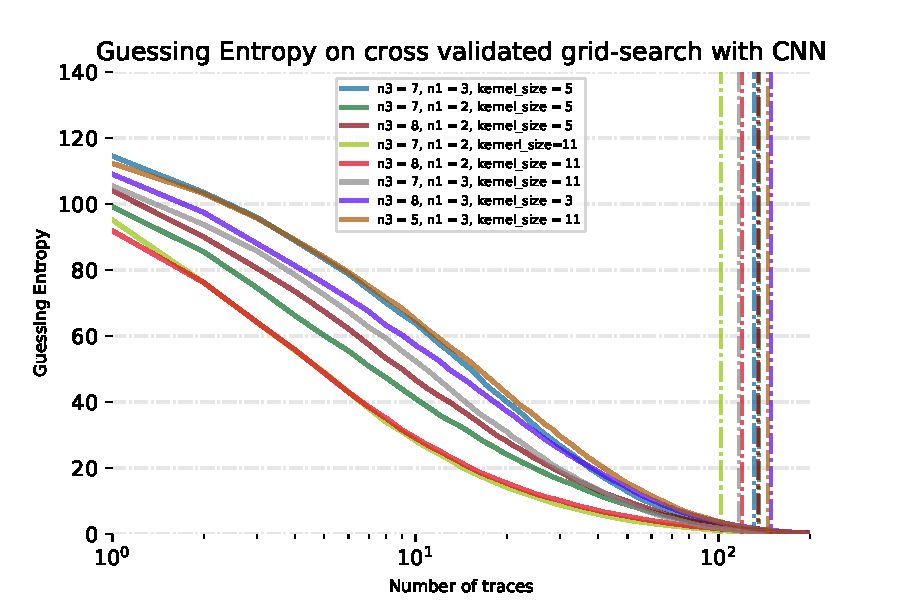
\includegraphics[width=\textwidth]{figures/ASCAD_700/with_mask_no_desynchro/GE_best_nodes}
        \caption{\gls{ge} for the \(8\) best architectures.}
        \label{table:ge_masking_perf}
    \end{subfigure}
    \caption{Results of Exp.~3 with Boolean secret-sharing.}
    \label{table:ge_masking}
\end{table}


For the selected architectures, our first attempt to use \gls{gv} did not give full satisfaction.
As an illustration, \autoref{fig:overfitting_peaks} presents it for one of the tested architectures -- averaged over the \(5\) folds of the cross-validation.
Indeed, it looks difficult to distinguish \glspl{poi}, \ie{} those identified by our \gls{snr} characterization, see \autoref{fig:vbp_masking_snr}, from \emph{ghost} peaks, \ie{} peaks \textit{a priori} independent of the sensitive target.
To explain this phenomenon, we decided to study the validation loss of the trained models.
\autoref{fig:overfitting_loss} presents it for one model and for each of the \(5\) cross-validation folds \(\mathrm{CV}_i$, $i\in \llbracket 0, 4 \rrbracket\).

\begin{figure}
    \centering
    \begin{subfigure}[]{0.49 \textwidth}
        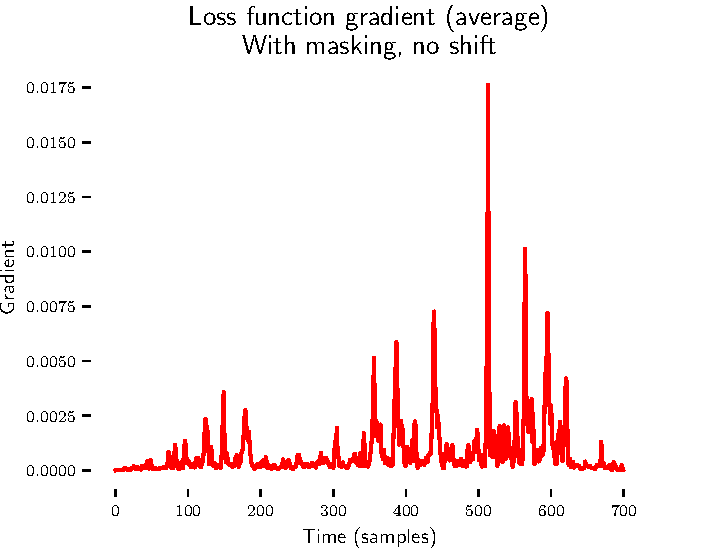
\includegraphics[width=\textwidth]{figures/ASCAD_700/with_mask_no_desynchro/VBP_Node_6191_without_early_stopping_review}
        \caption{\gls{gv} in presence of secret-sharing (without early-stopping).}
        \label{fig:overfitting_peaks}
    \end{subfigure}
    \begin{subfigure}[]{0.49 \textwidth}
        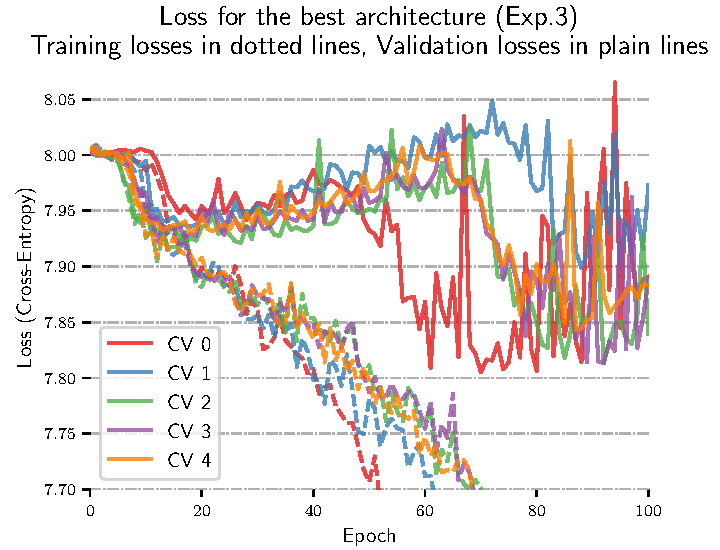
\includegraphics[width=\textwidth]{figures/ASCAD_700/with_mask_no_desynchro/Xent_Node_6191_review}
        \caption{Validation loss for each fold.}
        \label{fig:overfitting_loss}
    \end{subfigure}
	\caption{Explaining the ghost peaks.}
	\label{fig:overfitting}
\end{figure}

It may be observed in \autoref{fig:overfitting_loss} that the training and validation loss curves proceeded a fast big decrease after an initial plateau during the first \(15\) epochs.
After that, the validation loss starts increasing while the training loss still decreases.
After roughly \(50\) epochs, the validation loss goes on a regime with unstable results, but still higher than the training loss.
These observations are clues of over-fitting.%
\footnote{
    We recall the reader that an explanation of over-fitting has been given in \autoref{sec:results_exp}.
}
It means that the model exploits (non-informative) leakage not localized in the \glspl{poi} to memorize the profiling data and to improve the training loss.
Such a strategy should not generalize well on the validation traces.
As we are looking for models that implement a strategy that are generalizable on unseen traces, we propose to use a regularization technique called \emph{early-stopping}~\cite{goodfellow_deep_2017}: the training is stopped after a number of epochs called \emph{patience} -- in our case \(10\) -- if no remarkable decrease -- \ie{} up to a 
\emph{tolerance term}, \(0.25\) bits here -- is observed in the validation loss. 
With this slight modification, the previous architectures are trained again from scratch, and a better \gls{gv} is produced -- see \autoref{fig:vbp_masking_gv}.
As the main peaks are separated enough, an evaluator may conclude that they represent different leakages.

\begin{figure}
    \centering
    \begin{subfigure}{0.49 \textwidth}
        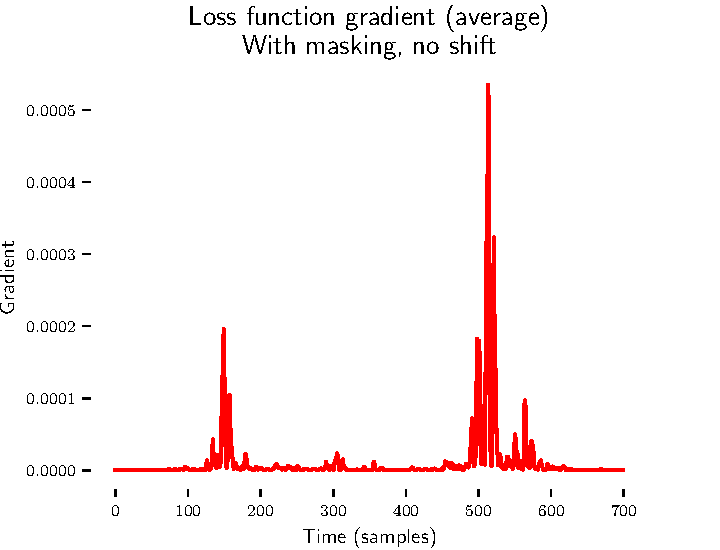
\includegraphics[width=\textwidth]{figures/ASCAD_700/with_mask_no_desynchro/VBP_Node_6191_review}
        \caption{\gls{gv}.}
        \label{fig:vbp_masking_gv}
    \end{subfigure}
    \begin{subfigure}{0.49 \textwidth}
        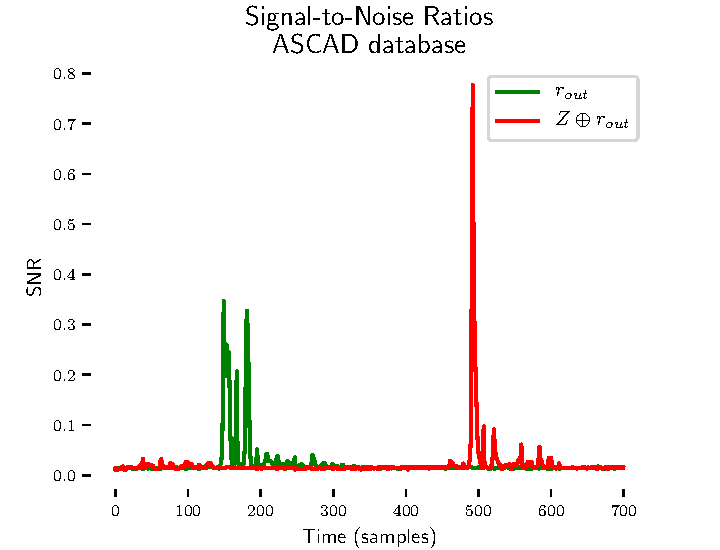
\includegraphics[width=\textwidth]{figures/ASCAD_700/snr_m_and_zxm}
        \caption{The corresponding \gls{snr} when taking \(\rout\) as a share.}
        \label{fig:vbp_masking_snr}
    \end{subfigure}
    \begin{subfigure}{0.49 \textwidth}
        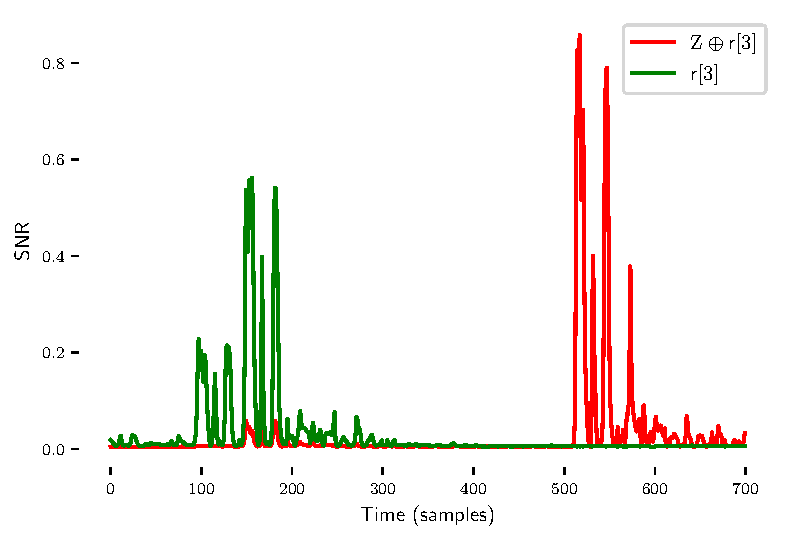
\includegraphics[width=\textwidth]{figures/ASCAD_700/snr_r3}
        \caption{The corresponding \gls{snr} when taking \(\M[3]\) as a share.}
        \label{fig:vbp_masking_snr_r3}
    \end{subfigure}
	\caption{Early-stopping is applied.}
	\label{fig:vbp_masking}
\end{figure}

\subsection{Comparison in the Context of Template Attacks}
\label{sec:comparison_with_snr}
A careful observation of \autoref{fig:vbp_masking} shows that the main peaks given by the \gls{gv} are not exactly aligned with those given by the \gls{snr} characterization -- performed under the hypothesis that the shares are known.
For \gls{gv}, the main peak appears at the points corresponding to the \(20\)-th clock cycle, which is one cycle after the one previously targeted by both the \gls{gv} and the \gls{snr} in the previous case where no counter-measure was considered -- see \autoref{sec:no_mask_no_desynchro}.
We validated that this phenomenon occurred for every successful visualization produced by \gls{gv}. 
Furthermore, concerning the peaks related to the mask leakage, the \gls{gv} only emphasizes one clock cycle (the \(6\)-th) whereas the \gls{snr} highlights two of them: the \(6\)-th and the \(7\)-th.
It implies that the \gls{gv} should not be taken as an exact equivalent to the \gls{snr}.

% Interpretation hypothesis
Actually, we found out a possible track of explanation to justify this slight shift by looking at the pseudo-code sketching the secret-sharing scheme of the \gls{ascad} database~\cite[Alg.~1]{prouff_study_2018}.
Indeed, the latter one emphasizes that another random variable forming a \(2\)-sharing of the output of \(\Sbox\), denoted as \(\mathsf{r}[3]\), is used in the scheme to protect the sensitive computation before and after applying the \(\sub{}\) operation, while the share \(\rout\) considered to compute the \gls{snr} in Figures \ref{fig:charac_ascad_snr} and \ref{fig:vbp_masking_snr} is used during the \(\sub{}\) operation.
By computing the \glspl{snr} of \(\Z \plusgf \mathsf{r}[3]\) and \(\mathsf{r}[3]\) in \autoref{fig:vbp_masking_snr_r3}, we remark that the peaks of \gls{snr} fit better with the peaks of \gls{gv} previously highlighted in the discussion.


Hence a question through this observation: does it have a sense for the trained \gls{cnn} to focus more on the leakages of the couple \((\Z \plusgf \mathsf{r}[3], \mathsf{r}[3])\) than on the leakages of the couple \((\Z \plusgf \rout, \rout)\)?
To give an answer, we decided to use our characterization method as a pre-processing for a Template Attack, and compare it to two pre-processing methods: \gls{snr} -- through \glspl{poi} selection -- and  \gls{pca} -- through dimensionality reduction.
The input dimension of the traces are reduced to \(2^n, n \in \{1, 2, 3, 4, 5\}\) points, based on the following methods:
\begin{itemize}
	\item \textbf{\gls{snr} strategy}: the \(2^{n-1}\) highest \glspl{poi} from the \gls{snr} of \(\rout\) and the \(2^{n-1}\) highest \glspl{poi} from the \gls{snr} of \(\Z \plusgf \rout\) are selected;
	\item \textbf{\gls{pca} strategy}: the \(2^n\) first components in a decreasing order of contribution are selected; 
	\item \textbf{\gls{gv} strategy}: the \(2^{n-1}\) highest \glspl{poi} from the \gls{gv} are selected from the area around the \(6\)-th clock cycle.
    Likewise, the other half comes from the peaks in the area around the \(20\)-th clock cycle.
\end{itemize}

\begin{remark}
    To make a fair comparison in the context of a first order secret-sharing, we assume that we know the shares during the characterization phase for \gls{snr}, so that we can localize the corresponding \glspl{poi}.
    Notice that we do not assume the mask knowledge neither during the profiling phase nor for the other strategies.
    Moreover, we do not use any re-combination function as described in \autoref{sec:PoIs} in none of the different strategies.

    Obviously, this scenario is not realistic as if one has access to the mask during characterization, then the latter one is very likely to be also available during the profiling phase.
\end{remark}


Once reduced, the traces are processed with a \gls{gta}, and the \gls{ge} is estimated.
The results are given on Figure~\ref{fig:ta_pois}. 
The plain curves denote the \gls{ge} for \gls{gv} whereas the dotted curves denote either \gls{ge} obtained with \gls{snr} (left) or \gls{pca} (right).

\begin{figure}
	\centering
    \begin{subfigure}{0.49 \textwidth}
        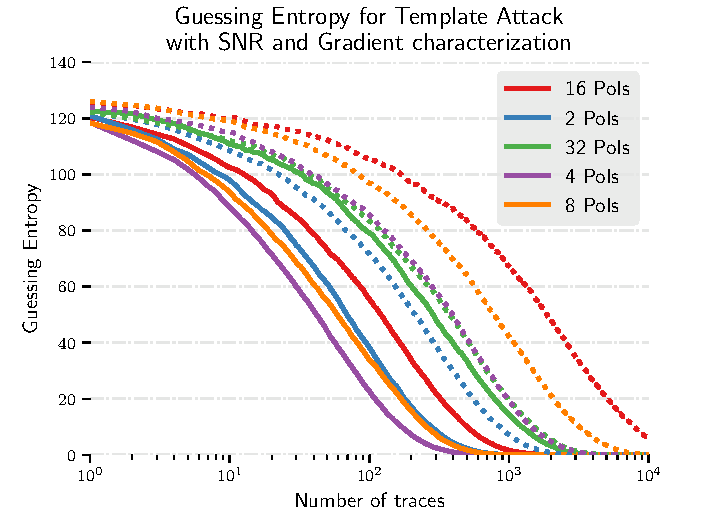
\includegraphics[width=\textwidth]{figures/ASCAD_700/with_mask_no_desynchro/GE_VBP_SNR_review}
        \caption{\ldots \gls{snr} based attacks.}
        \label{fig:ta_pois_snr}
    \end{subfigure}
    \begin{subfigure}{0.49 \textwidth}
        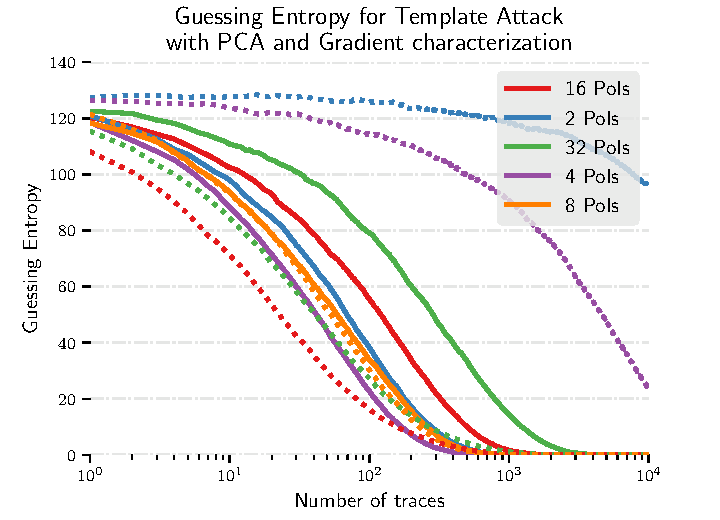
\includegraphics[width=\textwidth]{figures/ASCAD_700/with_mask_no_desynchro/GE_VBP_PCA_review}
        \caption{\ldots \gls{pca} based attacks.}
        \label{fig:ta_pois_pca}
    \end{subfigure}
	\caption{Comparison of the \gls{ge} for \gls{gv} based attacks in plain lines and, in dotted lines, \ldots}
	\label{fig:ta_pois}
\end{figure}

% Observations
From Figure~\ref{fig:ta_pois} we can observe several things:
\begin{itemize}
	\item Only a few \glspl{poi} from the \gls{gv} strategy are needed to get a successful attack.
	The optimal number of extracted \glspl{poi} is 4.
    Beyond that, the other \glspl{poi} bring more difficulty in the Template Attack than they bring new information (due to the increasing dimensionality).
	\item When the \gls{snr} strategy is applied, the optimal attack is done with 2 \glspl{poi} and the more \glspl{poi} are used, the less efficient are the attacks.
	This observation confirms that \gls{snr} selects relevant \glspl{poi} as expected. 
	However, when comparing the \gls{snr} and \gls{gv} strategies with a same number of \glspl{poi}, the latter one appears to be always better, except for 32 \glspl{poi} where both strategies seem equal.
	\item The \gls{pca} strategy does not work well for the two or four first extracted components.
    However, when considering eight components and above, it achieves an efficiency as good as the \gls{gv} strategy, and even sometimes better.
	\item In any case, the Template Attacks need much more traces to get a \gls{ge} converging towards zero than the best \gls{cnn} attack presented in Table~\ref{table:ge_masking}.
\end{itemize}

% First conclusion
Based on the presented experiments, we may draw several conclusions on the \gls{gv} efficiency.
First of all, it seems to be an accurate characterization method, almost always much better than that based on an \gls{snr}.
This first conclusion enables to answer the question previously asked: the targeted \glspl{poi} in \gls{gv} are relevant leakages and the couple of shares \((\Z \plusgf \mathsf{r}[3], \mathsf{r}[3])\) leaks more informative clues in the traces about the sensitive variable \(\Z\) than the couple of shares \((\Z \plusgf \rout, \rout)\).
Actually, this finding is not very surprising, since it could have been deduced from the \glspl{snr} computed by Benadjila \etal{} when presenting the \gls{ascad} database~\cite{prouff_study_2018}.
However, since the knowledge of the random shares is not required to train the \gls{cnn}, the attacker does not have to previously decide which sensitive intermediate computation is the most likely to lead to the most efficient attack.

% Second conclusion
Secondly, \gls{gv} can be used as a reliable dimensionality reduction pre-processing in presence of counter-measures, even more reliable than \gls{pca} in our cases where one makes a reduction to a very few dimensions (2 or 4).
However, this conclusion has a minor interest, as the \gls{gv} seen as a pre-processing method is done \textit{post-mortem}, and the training of a \gls{cnn} model did not suffer from a high dimensional input.

% Weakness
Last, but not least, the \gls{gv} method unfortunately faces a drawback: if the trained \gls{cnn} overfits, then the \gls{gv} might suffer from the presence of ghost peaks.
That is why the overfitting must be carefully monitored.
In this sense, visualizing the gradient can hopefully help to assess whether it is the case or not.

\subsection{Gradient Visualization on the Polymorphism Dataset}
    \label{sec:gv_claps}
    %%%%%%%%%%%%%%%%%%%%%%%%%%%%%%%%%%%%%%%%%%%%%%%%%%%%%%%%%%%%%%%%%%%%%%%%%%%%%%%%
%						GRADIENT VISUALIZATION ON CHAPTER 6 				   %
%%%%%%%%%%%%%%%%%%%%%%%%%%%%%%%%%%%%%%%%%%%%%%%%%%%%%%%%%%%%%%%%%%%%%%%%%%%%%%%%
As a final demonstration of the technique, we now apply \gls{gv} on the trained \glspl{cnn} from the two attacks \attCNN{} described in \autoref{sec:cnn_archi_esorics}, in order to show how this characterization method can provide insights about the acquired traces and the behavior of the target device.
For completeness, we additionnaly trained \glspl{cnn} targeting the remaining bytes of the secret key which have not been investigated yet for the attacks \attCNN{} in \autoref{chap:dl_sca_practice}.
The architecture used for those additional trainings remained exactly the same, namely:
\begin{equation}\label{eq:vgg_archi_esorics_grad}
	\softmax \circ \linLayer_{\card{\sensVarSet}} \circ [\actLayer \circ \linLayer_\linSize]^{n_1}
	\circ [\poolLayer_\pstride \circ \actLayer \circ \BNLayer \circ \convLayer_{\ksize, \numFilters}]^{n_2} \circ \BNLayer \enspace ,
\end{equation}
where \(\convLayer_{\ksize, \numFilters}\) denotes a convolutional layer made of \(\numFilters\) filters of size \(\ksize\), \(\BNLayer\) denotes a batch-normalization layer, \(\actLayer\) denotes the \gls{relu} activation function, \(\poolLayer_{\pstride}\) denotes an average pooling layer of size \(\pstride\), \(\linLayer\) denotes a dense layer, and \(\softmax\) denotes the softmax layer.
The hyper-parameters are given in \autoref{table:cnn_archi}.

\paragraph{\mbedTLS{}}
\autoref{fig:grad_mbed} shows the gradient visualizations applied on one trace from the \mbedTLS{} dataset based on the corresponding trained \gls{cnn}.
The top plot shows a trace whereas the bottom plots show the 16 gradients computed from this trace, targeting each byte.
Those gradients have been gathered into four pools.
\begin{figure}
	\centering
	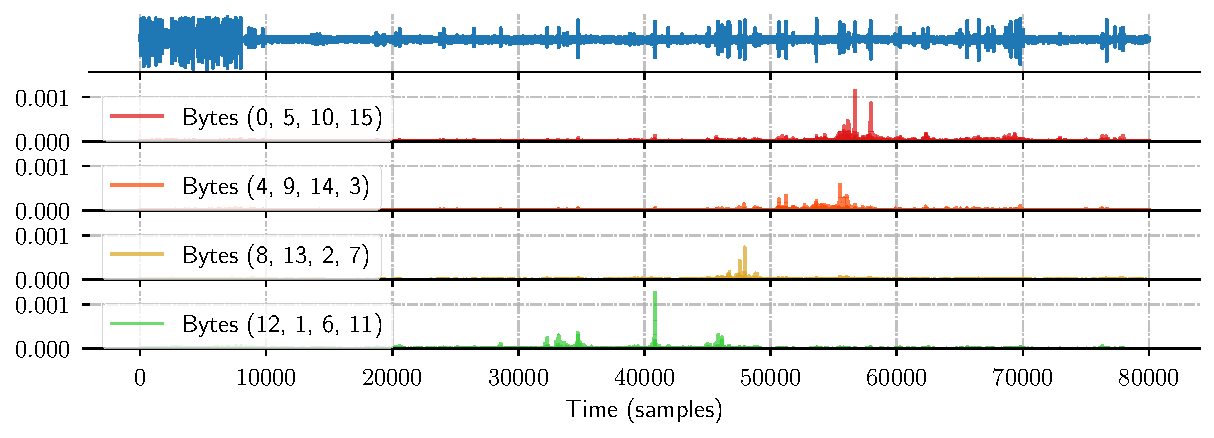
\includegraphics[width=\textwidth]{../Chapter6/Figures/grad_viz/v1/grads}
	\caption{\gls{gv} for one trace of the \mbedTLS{} implementation.}
	\label{fig:grad_mbed}
\end{figure}
First, it can be remarked that contrary to the \gls{snr} plotted in \autoref{fig:observations_v1}, the \gls{gv} shows some peaks in the different gradients plotted in \autoref{fig:grad_mbed}, which shows that the \gls{gv} is able to emphasize the \glspl{poi} despite the application of code polymorphism on the target implementation.

More particularly, it may be seen that the peaks of gradient corresponding to the bytes \((12, 1, 6, 11)\) colored in green appear first, followed by those of the bytes \((8, 13, 2, 7)\) in yellow, then those of the bytes \((4, 9, 14, 3)\) in orange and finally the peaks of gradient for the bytes \((0, 5, 10, 15)\) in red.
Interestingly, this order can be read in light of the source code of the implementation.
The \gls{aes} state is represented here by four \verb+uint32_t+ variables \verb+X0+, 
\ldots, \verb+X3+, each one denoting one column of the state array.
The repartition of the bytes into the state is represented in \autoref{fig:aes_state} at two steps of the first round which could potentially be the leakage source.
\begin{figure}
	\begin{subfigure}{0.49 \textwidth}
		\centering
		\begin{tikzpicture}[scale=0.5]
    \draw[fill=ceared!20] (0,3) rectangle node {\scriptsize 0} +(0.8,1);
    \draw[fill=cealime!20] (0,2) rectangle node {\scriptsize 1} +(0.8,1);
    \draw[fill=ceagold!20] (0,1) rectangle node {\scriptsize 2} +(0.8,1);
    \draw[fill=ceaorange!20] (0,0) rectangle node {\scriptsize 3} +(0.8,1);
    \draw[fill=ceaorange!20] (1,3) rectangle node {\scriptsize 4} +(0.8,1);
    \draw[fill=ceared!20] (1,2) rectangle node {\scriptsize 5} +(0.8,1);
    \draw[fill=cealime!20] (1,1) rectangle node {\scriptsize 6} +(0.8,1);
    \draw[fill=ceagold!20] (1,0) rectangle node {\scriptsize 7} +(0.8,1);
    \draw[fill=ceagold!20] (2,3) rectangle node {\scriptsize 8} +(0.8,1);
    \draw[fill=ceaorange!20] (2,2) rectangle node {\scriptsize 9} +(0.8,1);
    \draw[fill=ceared!20] (2,1) rectangle node {\scriptsize 10} +(0.8,1);
    \draw[fill=cealime!20] (2,0) rectangle node {\scriptsize 11} +(0.8,1);
    \draw[fill=cealime!20] (3,3) rectangle node {\scriptsize 12} +(0.8,1);
    \draw[fill=ceagold!20] (3,2) rectangle node {\scriptsize 13} +(0.8,1);
    \draw[fill=ceaorange!20] (3,1) rectangle node {\scriptsize 14} +(0.8,1);
    \draw[fill=ceared!20] (3,0) rectangle node {\scriptsize 15} +(0.8,1);	

    \draw (0.4,-1) node {\scriptsize \verb+X0+};
    \draw (1.4,-1) node {\scriptsize \verb+X1+};
    \draw (2.4,-1) node {\scriptsize \verb+X2+};
    \draw (3.4,-1) node {\scriptsize \verb+X3+};
\end{tikzpicture}
		\caption{\gls{aes} state after the first \ark{}}
		\label{fig:aes_state_ark}
	\end{subfigure}
	\begin{subfigure}{0.49 \textwidth}
		\centering
		\begin{tikzpicture}[scale=0.5]
    \draw[fill=ceared!20] (0,3) rectangle node {\scriptsize 0} +(0.8,1);
    \draw[fill=ceared!20] (0,2) rectangle node {\scriptsize 5} +(0.8,1);
    \draw[fill=ceared!20] (0,1) rectangle node {\scriptsize 10} +(0.8,1);
    \draw[fill=ceared!20] (0,0) rectangle node {\scriptsize 15} +(0.8,1);
    \draw[fill=ceaorange!20] (1,3) rectangle node {\scriptsize 4} +(0.8,1);
    \draw[fill=ceaorange!20] (1,2) rectangle node {\scriptsize 9} +(0.8,1);
    \draw[fill=ceaorange!20] (1,1) rectangle node {\scriptsize 14} +(0.8,1);
    \draw[fill=ceaorange!20] (1,0) rectangle node {\scriptsize 3} +(0.8,1);
    \draw[fill=ceagold!20] (2,3) rectangle node {\scriptsize 8} +(0.8,1);
    \draw[fill=ceagold!20] (2,2) rectangle node {\scriptsize 13} +(0.8,1);
    \draw[fill=ceagold!20] (2,1) rectangle node {\scriptsize 2} +(0.8,1);
    \draw[fill=ceagold!20] (2,0) rectangle node {\scriptsize 7} +(0.8,1);
    \draw[fill=cealime!20]  (3,3) rectangle node {\scriptsize 12} +(0.8,1);
    \draw[fill=cealime!20] (3,2) rectangle node {\scriptsize 1} +(0.8,1);
    \draw[fill=cealime!20] (3,1) rectangle node {\scriptsize 6} +(0.8,1);
    \draw[fill=cealime!20] (3,0) rectangle node {\scriptsize 11} +(0.8,1);	

    \draw (0.4,-1) node {\scriptsize \verb+X0+};
    \draw (1.4,-1) node {\scriptsize \verb+X1+};
    \draw (2.4,-1) node {\scriptsize \verb+X2+};
    \draw (3.4,-1) node {\scriptsize \verb+X3+};
\end{tikzpicture}
		\caption{\gls{aes} state at the end of the \sr{}}
		\label{fig:aes_state_mc}
	\end{subfigure}
	\caption{\gls{aes} states at two moments in the first round potentially leaking information about the secret key bytes.}
	\label{fig:aes_state}
\end{figure}
\autoref{fig:aes_state_ark} denotes the state after the first \ark{} while \autoref{fig:aes_state_mc} denotes the state at the end of the \sr{}.
Since the operations are done column-wise, the bytes belonging to the same column of the state should leak at close time samples to each other in the trace.
That being said, we easily remark that the pools of gradient peaks described above coincide with the columns of the \gls{aes} state at the end of the \sr{} depicted in \autoref{fig:aes_state_mc}, which corresponds to the call of the \glspl{lut} of the T-table implementation, rather than the key addition.

\paragraph{\aeshuitbit{}}
\begin{figure}
	\centering
	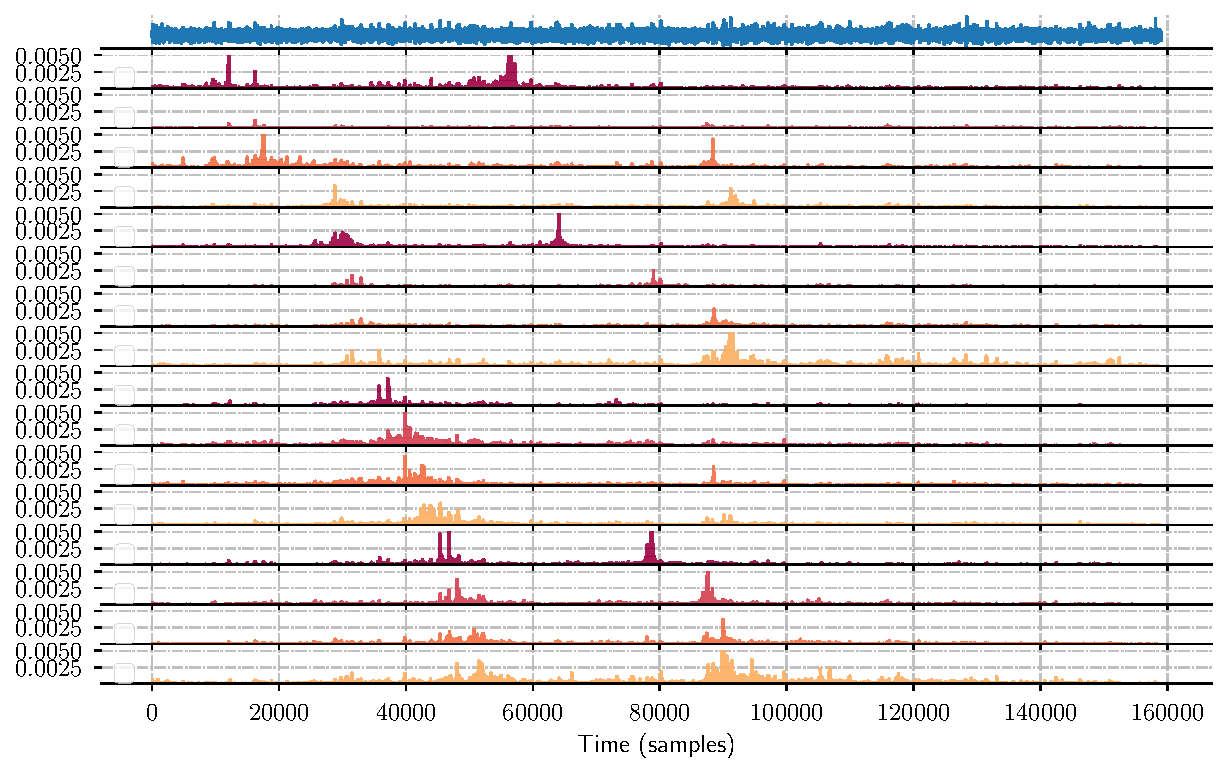
\includegraphics[width=\textwidth]{../Chapter6/Figures/grad_viz/v2/grads}
	\caption{\gls{gv} for one trace of the \aeshuitbit{} implementation.
	The top plot depicts the considered trace, whereas the bottom plots denote
	the gradients for each targeted byte.}
	\label{fig:grad_aes8bit}
\end{figure}
\autoref{fig:grad_aes8bit} shows the gradient visualizations in the same way as for \mbedTLS{}, but this time, for each key byte separately.
A focus on the first peak of each gradient highlights that they appear in increasing order of the byte index: the leakage probably comes from a \verb+for+ loop iterating over each byte of the \gls{aes} state.
Thus, the corresponding operation might be either \ark{} or \sub{}.
Furthermore, a close look at the second peak of each gradient reveals that they are almost aligned, except four of them: \((0, 4, 8, 12)\).
A quick look at the \sr{} operation inside the source code of the \aeshuitbit{} implementation reveals that it never manipulates the latter bytes of the state, contrary to the others.
This can also be deduced from \autoref{fig:aes_state} where the only bytes not moving from \autoref{fig:aes_state_ark} to \autoref{fig:aes_state_mc} are those same bytes.
We deduce that for the bytes \(0, 4, 8, 12\), the \gls{cnn} exploits the joint leakages of the \ark{} and \sub{} operations, whereas for the other bytes the \gls{cnn} rather exploits the joint leakages of the \ark{} and \sr{} operations.

Anyway, in every cases, two leakages are jointly exploited by the \gls{cnn} in the \aeshuitbit{} implementation whereas only one leakage seems to be used in the \mbedTLS{} one.
This might explain why the attack on the latter implementation is slightly worse than in the former implementation, although the traces seemed less noisy at first sight. 

Finally, the gradient visualizations showed in both \autoref{fig:grad_mbed} and \autoref{fig:grad_aes8bit} highlight relatively sharp peaks.%
\footnote{A similar analysis can be done on other traces from the dataset.}
This means that the \gls{cnn} model is able to precisely localize the leakages in the traces, despite the application of code polymorphism.
In other words, the code transformations applied here did not prevent the \gls{cnn} model to localize and exploit the leakage.
Instead, one would expect sound code transformations to flatten and spread the gradient peaks along a wider zone of the trace, in order to increase uncertainty about the leakage localization.
One might imagine other code transformations which could be plugged in the Belleville \etal{}'s tool in order to address this problem, although beyond the scope of this demonstration.

\section{Conclusion}
    %%%%%%%%%%%%%%%%%%%%%%%%%%%%%%%%%%%%%%%%%%%%%%%%%%%%%%%%%%%%%%%%%%%%%%%%%%%%%%%%
%                       CONCLUSION CHAPTER 7                                   %
%%%%%%%%%%%%%%%%%%%%%%%%%%%%%%%%%%%%%%%%%%%%%%%%%%%%%%%%%%%%%%%%%%%%%%%%%%%%%%%%
In this chapter, we have theoretically shown that a method called \glsfirst{gv} can be used to localize \glsfirstplural{poi}.
This result relies on two assumptions considered as realistic in an \gls{sca} context. 


Generally, the efficiency of the proposed method only depends on the ability of the profiling model to succeed in the attack.
In the case where counter-measures like secret-sharing or misalignment are considered, \glspl{cnn} are shown to still build good \gls{pmf} estimations, and thereby the \gls{gv} provides a good characterization tool.
In addition, such a visualization can be made for each trace individually, and the method does not require more work than needed to perform a profiling with \glspl{cnn} leading to a successful attack.
Therefore, characterization can be done after the profiling phase whereas profiling attacks with \glsfirstplural{gta} often require to proceed a preliminary characterization phase.

We verified the efficiency of our proposed method on simulated data.
It has been shown that as long as a \gls{dnn} is able to have slightly better performance than randomness, it can localize points containing the informative leakage. 

On experimental traces, we have empirically shown that \gls{gv} is at least as good as the state-of-the-art characterization methods, in different cases corresponding to the presence or not of different counter-measures.
Not only it can still localize \glspl{poi} in presence of de-synchronization or secret-sharing but it has also been shown that different \glspl{poi} can be emphasized compared to the first ones highlighted by \gls{snr}.
These new \glspl{poi} have been shown to be at least as relevant as the ones proposed by \gls{snr}.

Altogether, the gradient visualization method we proposed here provides tools to the evaluator in order to get a clear understanding of the leakage detected by the \glspl{dnn} during the profiling phase.
We have shown how this characterization could be combined with information on the source code on order to better identify the vulnerability in the code.
Therefore, those insights can not only help the evaluator to build its diagnosis, but also help the developer to fix the vulnerability of implementations, no matter they are originally protected or not.
